\documentclass[compress]{beamer}

\usepackage[nofonts]{ctex}
\setCJKmainfont[ItalicFont={Kaiti SC}]{Kaiti SC}%
%\setCJKmainfont[ItalicFont={AR PL KaitiM GB}]{AR PL KaitiM GB}%
%\setCJKsansfont{WenQuanYi Zen Hei}% 文泉驿的黑体

\mode<beamer>
{
     \useinnertheme{rectangles}
     %\useoutertheme{infolines}
     %\useoutertheme{split}
     \usecolortheme{rose}
     \usecolortheme{seahorse}

     \setbeamertemplate{navigation symbols}{}%remove navigation symbols

     %\expandafter\def\expandafter\insertshorttitle\expandafter{%
     %\insertshorttitle\hfill%
     %\insertframenumber\,/\,\inserttotalframenumber}
     %\raisebox{-1ex}{\includegraphics[width=3ex]{Overlays/logo.pdf}}}

    \setbeamertemplate{footline} {
      \leavevmode%
      \hbox{%
      \begin{beamercolorbox}[wd=.1\paperwidth,ht=2.25ex,dp=1ex,left]{date in head/foot}%
        \usebeamerfont{date in head/foot}%
        \hspace*{1ex}\raisebox{-0.8ex}{\includegraphics[width=3ex]{Overlays/logo.pdf}}%
      \end{beamercolorbox}%
      \begin{beamercolorbox}[wd=.4\paperwidth,ht=2.25ex,dp=1ex,right]{date in head/foot}%
        \usebeamerfont{date in head/foot}\insertsection\hspace*{1ex}
      \end{beamercolorbox}%
      \begin{beamercolorbox}[wd=.4\paperwidth,ht=2.25ex,dp=1ex,left]{date in head/foot}%
        \usebeamerfont{date in head/foot}\hspace*{1ex}\insertsubsection
      \end{beamercolorbox}%
      \begin{beamercolorbox}[wd=.1\paperwidth,ht=2.25ex,dp=1ex,right]{date in head/foot}%
        \insertframenumber{} / \inserttotalframenumber\hspace*{1ex}
      \end{beamercolorbox}}%
      \vskip0pt%
    }

}

%\defbeamertemplate*{footline}{mytheme}
%{
%  \leavevmode%
%  \hbox{%
%  \begin{beamercolorbox}[wd=.5\paperwidth,ht=2.25ex,dp=1ex,center]{author in head/foot}%
%    \usebeamerfont{author in head/foot}\insertshortauthor~~%
%    \raisebox{-1ex}{\includegraphics[width=3ex]{Overlays/logo.pdf}}%
%  \end{beamercolorbox}%
%  \begin{beamercolorbox}[wd=.5\paperwidth,ht=2.25ex,dp=1ex,right]{title in head/foot}%
%    \usebeamerfont{title in head/foot}\insertshorttitle{}\hspace*{2em}
%    \insertframenumber{} / \inserttotalframenumber\hspace*{2ex} 
%  \end{beamercolorbox}}%
%  \vskip0pt%
%}
%\usebeamertemplate{mytheme}

%\setbeamercovered{transparent}

\mode<handout>
{
	\usetheme{default}
	\usepackage{pgfpages}
	\pgfpagesuselayout{4 on 1}[a4paper,landscape,border shrink=5mm]
}


\usepackage{amsmath,latexsym,amssymb,amsfonts,amsbsy}
\usepackage{graphicx}
\usepackage{array}
\usepackage{hyperref}
\usepackage{textpos}
\usepackage{color, colortbl}
\usepackage{fancybox}
\usepackage{comment}
\usepackage{tikz}
\usetikzlibrary{arrows, trees, shapes, positioning, arrows.meta}
\usepackage{tikz-uml}

\newcommand{\romannumber}[1]{{\textrm{\uppercase\expandafter{\romannumeral
#1}}}}

\setbeamercolor{dblue}{fg=white,bg=gray!70!blue} % for beamercolorbox
 \newenvironment{pblock}{\begin{beamercolorbox}[rounded=true,
          shadow=false]{dblue}}{\end{beamercolorbox}}
 \newenvironment{bblock}{\begin{beamercolorbox}[rounded=true,
          shadow=false]{fg=black, bg=white}}{\end{beamercolorbox}}

\graphicspath{{figure/}}

%%%%%%%%%%%%%%%%%%%%%%%%%%%%%%%%%%%%%%%%%%%%%%%%%%%%%%%%%%%%%%%%%
%    body                                                       %
%%%%%%%%%%%%%%%%%%%%%%%%%%%%%%%%%%%%%%%%%%%%%%%%%%%%%%%%%%%%%%%%%


\begin{document}

\AtBeginSection[]
{ 
    \begin{frame}<beamer> 
		\frametitle{内容提要} 
		\tableofcontents[currentsection,currentsubsection,
        subsectionstyle=show/shaded/hide] 
	\end{frame} 
} 

					
\title{第六章 ~~ 建立辅助模型}

\author[面向对象的分析与设计]
{曹东刚\\\href{mailto:caodg@pku.edu.cn}{caodg@pku.edu.cn}}

\institute[北京大学]{北京大学信息学院研究生课程 - 面向对象的分析与设计 \\
\href{http://sei.pku.edu.cn/~caodg/course/oo}{http://sei.pku.edu.cn/\~{}caodg/course/oo}}

\date{}

\titlegraphic{\includegraphics[height=0.10\textwidth]{Overlays/logo.pdf}}

\begin{frame}[plain]
	\titlepage
\end{frame}

\setcounter{framenumber}{0}

\begin{frame}
  \frametitle{类图与其他模型图的关系}

  \noindent\begin{tabular}{lp{4cm} p{3.2cm}} \hline
    方法 & 模型图 & 特点 \\ \hline\hline
  OMT     & 对象模型 + 动态模型 + 功能模型 & 掺杂其他方法 \\ \hline
  OOSE    & 需求模型 + 健壮模型 + 设计模型 & 解决不同阶段问题 \\ \hline
  Booch方法 & 基本模型 + 补充模型 & 以OO方法为核心 \\ \hline
  Coad/Yourdon &  类图 + 流程图 & 以OO方法为核心 \\ \hline
  UML & 收集了大量的模型图 & 从不同的视角对复杂系统建模 \\ \hline
\end{tabular}
\end{frame}

\begin{frame}
  \frametitle{UML2中的各种图}
\tikzstyle{abstract}=[rectangle, draw=black, 
        text centered, font=\itshape \footnotesize,  anchor=north, 
        text width=2cm]
\tikzstyle{diagram}=[rectangle, draw=black, 
        text centered, font=\footnotesize, anchor=north, , text width=2cm]
\tikzstyle{myarrow}=[->, >=open triangle 90, thick]
\tikzstyle{line}=[-, thick]

\noindent\resizebox{\hsize}{!} {%
\begin{tikzpicture}[node distance=2cm]
  \node (Diagram) [abstract, rectangle] { Diagram };
    \node (AuxNode02) [text width=0.5cm, below=1.5cm of Diagram] {};
    \node (Structure) [abstract, rectangle , left=of AuxNode02]
    { Structure \\[-1ex] Diagram};
    \node (Behaviour) [abstract, rectangle , right=of AuxNode02]
    { Behaviour \\[-1ex] Diagram };
        
    \node (AuxNode03) [below=1.5cm of Structure] {};
    \node (Profile) [diagram, rectangle , left=of AuxNode03, xshift=1cm]
    { Profile \\[-1ex] Diagram};
    \node (Component) [diagram, rectangle , right=of AuxNode03, xshift=-3cm]
    { Component \\[-1ex] Diagram};
    \node (Class) [diagram, rectangle , below=0.4cm of Profile]
    { Class \\[-1ex] Diagram };
    \node (Composite) [diagram, rectangle , below=0.4cm of Class]
    { Composite \\[-1.5ex] Structure \\[-1.5ex] Diagram };
    \node (Deployment) [diagram, rectangle , below=0.4cm of Component]
    { Deployment \\[-1ex] Diagram };
        
    \node (Package) [diagram, rectangle , right=of Component, xshift=-1.6cm]
    { Package \\[-1ex] Diagram};
    \node (Object) [diagram, rectangle , below=0.4cm of Package]
    { Object \\[-1ex] Diagram };

    \node (AuxNode04) [below=1.5cm of Behaviour] {};
    \node (Usecase) [diagram, rectangle , left=of AuxNode04, xshift=2cm]
    { Use Case \\[-1ex] Diagram };
    \node (Activity) [diagram, rectangle , right=of AuxNode04, xshift=-2cm]
    { Activity \\[-1ex] Diagram };
    \node (Interaction) [diagram, rectangle , below=0.4cm of Usecase]
    { Interaction \\[-1ex] Diagram };
    \node (State) [diagram, rectangle , below=0.4cm of Activity]
    { State Machine \\[-1.5ex] Diagram };

    \node (AuxNode05) [below=1.5cm of Interaction] {};
    \node (Timing) [diagram, rectangle , below=1.5cm of Interaction ]
    { Timing \\[-1ex] Diagram };
    \node (Sequence) [diagram, rectangle , left=0.4cm of Timing]
    { Sequence \\[-1ex] Diagram };
    \node (Communication) [diagram, rectangle , left=0.4cm of Sequence]
    { Communication \\[-1ex] Diagram };
    \node (Interover) [diagram, rectangle ,
    right=0.4cm of Timing.north east,anchor=north west]
    { Interaction \\[-1.5ex] Overview \\[-1.5ex] Diagram };

    \draw[myarrow] (Structure.north) -- ++(0,0.5) -| (Diagram.south);
    
    \draw[myarrow] (Profile.west) -- ++(-0.2,0) 
        -- ([yshift=0.5cm, xshift=-0.2cm] Profile.north west) 
        -| ([xshift=-0.0cm]Structure.south);
    \draw[line] (Class.west) -- ++(-0.2,0) -- ([xshift=-0.2cm] Profile.west) ; 
    \draw[line] (Composite.west) -- ++(-0.2,0) -- ([xshift=-0.2cm] Profile.west) ;

    \draw[myarrow] (Component.east) -- ++(0.2,0) 
        -- ([yshift=0.5cm, xshift=0.2cm] Component.north east) 
        -| ([xshift=0cm]Structure.south);
    \draw[line] (Deployment.east) -- ++(0.2,0) -- ([xshift=0.2cm] Component.east) ;
    \draw[line] (Package.west) -- ++(-0.2,0) ;
    \draw[line] (Object.west) -- ++(-0.2,0) ;
     
    \draw[myarrow] (Behaviour.north) -- ++(0,0.5) -| (Diagram.south);

    \draw[myarrow] (Usecase.west) -- ++(-0.2,0) 
      -- ([yshift=0.5cm, xshift=-0.2cm] Usecase.north west) 
      -| ([xshift=0cm]Behaviour.south);
    \draw[line] (Interaction.west) -- ++(-0.2,0) 
      -- ([xshift=-0.2cm] Usecase.west) ; 

    \draw[myarrow] (Activity.east) -- ++(0.2,0) 
      -- ([yshift=0.5cm, xshift=0.2cm] Activity.north east) -|
     ([xshift=-0cm]Behaviour.south);
    \draw[line] (State.east) -- ++(0.2,0) 
      -- ([xshift=0.2cm] Activity.east) ; 
     
    \draw[myarrow] (Sequence.north) -- ++(0,0.5) -| (Interaction.south);
    \draw[myarrow] (Communication.north) -- ++(0,0.5) -| (Interaction.south) ; 
    \draw[myarrow] (Timing.north) -- ++(0,0.5) -| (Interaction.south) ; 
    \draw[myarrow] (Interover.north) -- ++(0,0.5) -| (Interaction.south) ; 
\end{tikzpicture}
}
\end{frame}

\begin{frame}
  \frametitle{本书建模方法用类图作为主要模型}
  类图为基本模型,用况图为需求模型,其他模型图为辅助\\[2ex]

\resizebox{0.9\hsize}{!} {%
\tikzstyle{caption}=[font=\bfseries \small, align=center]
\tikzstyle{ntext}=[font=\small, align=center]
\begin{tikzpicture}
%  \draw [help lines, step=0.5cm] (0,0) grid (8,5) ;
  \draw (0,0) rectangle (8,1) ;
  \node [caption] at (4, 0.5) {模型规约} ;
  \draw (0,1.2) rectangle (1.5,5) ;
  \node [caption] at (0.75, 4.5) {需求模型} ;
  \node [ntext] at (0.75, 2.75) {用况图} ;
  \draw (6.5,1.2) rectangle (8,5) ;
  \node (ReqT) [caption] at (7.25, 4.5) {辅助模型} ;
  \node (PkgT) [below=0.5cm of ReqT, ntext] {包图} ;
  \node (SeqT) [below=0.1cm of PkgT, ntext] {顺序图} ;
  \node (ActT) [below=0.1cm of SeqT, ntext] {活动图} ;
  \node (EtcT) [below=0.1cm of ActT, ntext] {\dots} ;
  \draw (1.7,1.2) rectangle (6.3,5) ;
  \node (ClsT) [caption] at (4, 4.5) {基本模型:类图} ;
  \node (ObjL) [below=0.5cm of ClsT, text width=2cm, minimum
  height=0.6cm, rectangle, draw, xslant=0.6] {} ;
  \node (ObjT) [below=0.5cm of ClsT, ntext] {对象层} ;
  \node (FeaL) [below=0.2cm of ObjT, text width=2cm, minimum
  height=0.6cm, rectangle, draw, xslant=0.6] {} ;
  \node (FeaT) [below=0.2cm of ObjT, ntext] {特征层} ;
  \node (ReaL) [below=0.2cm of FeaT, text width=2cm, minimum
  height=0.6cm, rectangle, draw, xslant=0.6] {} ;
  \node (ReaT) [below=0.2cm of FeaT, ntext] {关系层} ;
\end{tikzpicture}
}
\end{frame}

\begin{frame}
  \frametitle{本书方法使用的各种UML图}

  \noindent\begin{tabular}{>{\arraybackslash}m{1.6cm}ll}
    \rowcolor{purple!20}
    类图 & 基本模型 & 最重要,必不可少 \\
    \rowcolor{cyan!20}
    用况图 & 需求模型 & 建模的基础,提倡使用 \\
    包图 & 辅助模型 & 系统规模较大时使用 \\
    顺序图 & 辅助模型 & 补充类图,在交互情况较复杂时使用 \\
    活动图 & 辅助模型 & 描述对象的操作流程,也可描述高层行为 \\
    状态机图 & 辅助模型 & 准确描述状态与行为复杂的对象 \\
    构件图与部署图 & 辅助模型 & 描述构件组织与部署方案 \\ 
    \rowcolor{gray!30}
    对象图与通信图 & & 不建议使用 \\ 
    \rowcolor{gray!30}
    其他 & & 无强烈建议
  \end{tabular}
\end{frame}

\section{包图}

\begin{frame}
\frametitle{包图定义}
\begin{block} {包(package)}
  是一种将其他模型元素组织起来,形成较大粒度的系统单位的通
  用机制 \\
  基本思想: 从不同粒度描述系统 --- G. Miller 的“7±2原则” 
\end{block}


  \alert{\textbf{注意}}:
  \begin{itemize}
    \item 包是一种组织机制而不是一种基本模型元素
    \item 包可以嵌套
    \item 包中的模型元素应具有某种意义的内在联系
    \item 包的划分有一定的灵活性或随意性  
  \end{itemize}
\end{frame}

\begin{frame}
  \frametitle{包的表示法}
  \begin{columns}
    \column{0.4\hsize}
  \resizebox{3cm}{!} {%
    \begin{tikzpicture}
    \node (Body) [minimum height=1cm, text width=2cm, text centered, draw, rectangle] { 名称 };
    %\draw (Body.north west) -- ++(0, +0.3cm) -- ++(+1.0cm, 0) -- ++(0, -0.3cm) ;
    \node [above = 0cm of Body.north west, anchor=south west, minimum height=0.2cm, text width=0.5cm, draw, rectangle] {};
  \end{tikzpicture}
  }

  \vspace*{1cm}

  \resizebox{3cm}{!} {%
    \begin{tikzpicture}
    \node (Body) [minimum height=1cm, text width=2cm, text centered,
    draw, rectangle] { 内容 };
    %\draw (Body.north west) -- ++(0, +0.3cm) -- ++(+1.0cm, 0) -- ++(0, -0.3cm) ;
    \node [above = 0cm of Body.north west, anchor=south west, 
      inner ysep=0.2ex,
      text width=0.5cm, draw, rectangle, font=\tiny] {名称};
  \end{tikzpicture}
  }
    \column{0.6\hsize}
  \resizebox{6cm}{!} {%
    \begin{tikzpicture}
    \node (Body) [minimum height=4cm, text width=6cm, text centered,
    draw, rectangle] {};
    %\draw (Body.north west) -- ++(0, +0.3cm) -- ++(+1.0cm, 0) -- ++(0, -0.3cm) ;
    \node (Name) [above = 0cm of Body.north west, anchor=south west, 
      %inner ysep=0.2ex,
      text width=1.5cm, draw, rectangle, font=\small] {教务管理};

    \node (Teacher) [below = 1.0cm of Name.south east, 
      %inner ysep=0.2ex,
      text width=1.0cm, draw, rectangle, font=\small] {教师};
    \node (Student) [below = 1.0cm of Teacher, 
      %inner ysep=0.2ex,
      text width=1.0cm, draw, rectangle, font=\small] {学生};

    \node (Body1) [right = 1.0cm of Teacher.south east, anchor=north west,
      minimum height=1cm, text width=2cm, text centered,
    draw, rectangle] {课程管理  };
    %\draw (Body.north west) -- ++(0, +0.3cm) -- ++(+1.0cm, 0) -- ++(0, -0.3cm) ;
    \node [above = 0cm of Body1.north west, anchor=south west, 
      minimum height = 0.2cm,
      text width=0.5cm, draw, rectangle, ] {};
  \end{tikzpicture}
  }

\end{columns}

\end{frame}

\begin{frame}
  \frametitle{包之间的关系及表示法}

  \only<1> {
\noindent  \alert{引入(import)}
  是包之间的一种依赖关系,表明源包中的模型元素能够\alert{直接}引用
  目标包中的模型元素
  \begin{itemize}
    \item 原由——名字空间(为了避免命名冲突)
    \item 以包为单位划分名字空间,引用时给出路径名
    \item 引入关系表明可以直接引用
  \end{itemize}

\noindent \alert{访问(access)}访问关系与引入关系类似,二者之间的差别:\\
UML1:目标包的元素是否可以被引入源包的其他包引入 \\
UML2:目标包(或目标元素)的可见性不同
}

  \only<2> {
  \noindent\resizebox{\hsize}{!} {%
    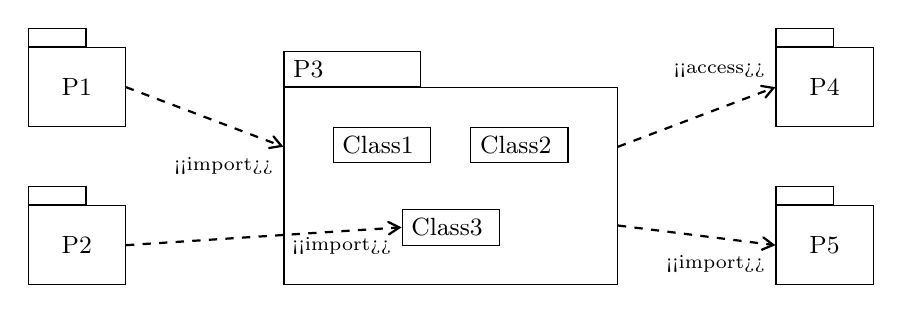
\begin{tikzpicture}
    \tikzstyle{PBody}=[font=\small, align=center, minimum height=1cm, text width=1cm, text centered, draw, rectangle]
    \tikzstyle{PName}=[font=\small, minimum height=0.2cm, text width=0.5cm, draw, rectangle]
    \tikzstyle{Depend}=[->, >=angle 60, thick, dashed]

    \node (Body) [minimum height=2.5cm, text width=4cm, text centered,
    draw, rectangle] {};
    \node (Name) [above = 0cm of Body.north west, anchor=south west, 
      text width=1.5cm, draw, rectangle, font=\small] {P3};

    \node (Class1) [below = 0.5cm of Name.south east, xshift=-0.5cm,
      text width=1.0cm, draw, rectangle, font=\small] {Class1};
    \node (Class2) [right = 0.5cm of Class1, 
      text width=1.0cm, draw, rectangle, font=\small] {Class2};
    \node (Class3) [above = 0.5cm of Body.south, 
      text width=1.0cm, draw, rectangle, font=\small] {Class3};

    \node (P1Body) [left = 2cm of Body.north west, PBody] { P1 };
    \node [above = 0cm of P1Body.north west, anchor=south west, PName] {};

    \node (P2Body) [left = 2cm of Body.south west, anchor=south east, PBody] { P2 };
    \node [above = 0cm of P2Body.north west, anchor=south west, PName] {};

    \node (P4Body) [right = 2cm of Body.north east, PBody] { P4 };
    \node [above = 0cm of P4Body.north west, anchor=south west, PName] {};

    \node (P5Body) [right = 2cm of Body.south east, anchor=south west, PBody] { P5 };
    \node [above = 0cm of P5Body.north west, anchor=south west, PName] {};

    \draw[Depend](P1Body.east) -- ([yshift=0.5cm]Body.west)
    node[font=\scriptsize, anchor=north east]{<<import>>} ;

    \draw[Depend] ([yshift=0.5cm]Body.east) -- (P4Body.west) 
    node[font=\scriptsize, anchor=south east]{<<access>>} ;

    \draw[Depend] ([yshift=-0.5cm]Body.east) -- (P5Body.west) 
    node[font=\scriptsize, anchor=north east]{<<import>>} ;

    \draw[Depend](P2Body.east) -- (Class3.west)
    node[font=\scriptsize, anchor=north east]{<<import>>} ;
 
  \end{tikzpicture}
  }
}

  \only<3> {
    \alert{合并(merge)} 是包之间的一个有向关系,表明目标包的概念定义被合并到源
    包中。建议对类给出完整的定义,不要分散到多个包中描述 \\[2ex]

  \resizebox{0.9\hsize}{!} {%
    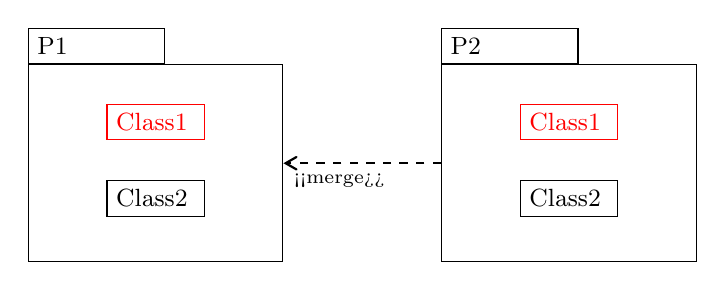
\begin{tikzpicture}
    \tikzstyle{Depend}=[->, >=angle 60, thick, dashed]
    \tikzstyle{Class}=[text width=1.0cm, draw, rectangle, font=\small]

    \node (P1Body) [minimum height=2.5cm, text width=3cm, text centered,
    draw, rectangle] {};
    \node (Name) [above = 0cm of P1Body.north west, anchor=south west, 
      text width=1.5cm, draw, rectangle, font=\small] {P1};

    \node (P1Class1) [below = 0.5cm of P1Body.north, Class, color=red] {Class1};
    \node (P1Class2) [below = 0.5cm of P1Class1.south, Class] {Class2};

    \node (P2Body) [minimum height=2.5cm, text width=3cm, text centered,
    draw, rectangle, right = 2cm of P1Body] {};
    \node (Name) [above = 0cm of P2Body.north west, anchor=south west, 
      text width=1.5cm, draw, rectangle, font=\small] {P2};

    \node (P2Class1) [below = 0.5cm of P2Body.north, Class, color=red] {Class1};
    \node (P2Class2) [below = 0.5cm of P2Class1.south, Class] {Class2};

    \draw[Depend](P2Body.west) -- (P1Body.east)
    node[font=\scriptsize, anchor=north west]{<<merge>>} ;
  \end{tikzpicture}
  }
  }

  \only<4> {
    \alert{包之间的其他关系}

    \alert{泛化}——没有正式的定义,只在包图的某些例子中出现

    \alert{依赖}——不加任何关键词的依赖关系,没有确切的定义
  }

\end{frame}

\begin{frame}
  \frametitle{如何建立包图}
  \only<1> {
      \begin{columns}
        \column{0.5\hsize}
  \begin{enumerate}
    \item 将模型元素打包
      \begin{enumerate}
        \item [a] 参照类图中的各种关系
          \begin{itemize}
            \item 一般-特殊结构 
            \item 整体-部分结构 
            \item 关联 
            \item 消息 
            \item 其他关系
          \end{itemize}
        \item [b] 根据问题域和用况
          \begin{itemize}
            \item 对象来源 
            \item 功能类别
            \item 通信频繁程度 
            \item 并发和分布情况
          \end{itemize}
      \end{enumerate}
  \end{enumerate}

        \column{0.5\hsize}

    \begin{enumerate}

      \item [c] 包的内容交叉问题
      \end{enumerate}

  \resizebox{4cm}{!} {%
    \begin{tikzpicture}
    \tikzstyle{PBody}=[font=\small, align=center, minimum height=1cm, text width=1cm, text centered, draw, rectangle]
    \tikzstyle{PName}=[font=\small, minimum height=0.2cm, text width=0.5cm, draw, rectangle]
    \tikzstyle{Depend}=[->, >=angle 60, thick, dashed]

    \node (Body) [minimum height=2cm, text width=4cm, text centered,
    draw, rectangle] {};
    \node (Name) [above = 0cm of Body.north west, anchor=south west, 
      text width=1.5cm, draw, rectangle, font=\small] {课程管理};

    \node (Class1) [below = 0.2cm of Name.south east, xshift=-0.5cm,
      text width=1.0cm, draw, rectangle, font=\small] {教师};
    \node (Class2) [right = 0.5cm of Class1, 
      text width=1.0cm, draw, rectangle, font=\small] {学生};
    \node (Class3) [above = 0.2cm of Body.south, 
      text width=1.0cm, draw, rectangle, font=\small] {课程};
  \end{tikzpicture}
  }

  \vspace*{0.3cm}
  \resizebox{4cm}{!} {%
    \begin{tikzpicture}
    \tikzstyle{PBody}=[font=\small, align=center, minimum height=1cm, text width=1cm, text centered, draw, rectangle]
    \tikzstyle{PName}=[font=\small, minimum height=0.2cm, text width=0.5cm, draw, rectangle]
    \tikzstyle{Depend}=[->, >=angle 60, thick, dashed]

    \node (Body) [minimum height=2.2cm, text width=4cm, text centered,
    draw, rectangle] {};
    \node (Name) [above = 0cm of Body.north west, anchor=south west, 
      text width=1.5cm, draw, rectangle, font=\small] {学籍管理};

    \node (Class1) [below = 0.2cm of Name.south east, xshift=-0.5cm,
      text width=1.0cm, draw, rectangle, font=\small] {学历};
    \node (Class2) [right = 0.5cm of Class1, 
      text width=1.0cm, draw, rectangle, font=\small] {学位};
    \node (Class3) [above = 0.2cm of Body.south, 
      text width=1.5cm, text centered, draw, rectangle, font=\small] {<<副本>>
      \\[-1ex] 学生};
  \end{tikzpicture}
  }
\end{columns}
}

  \only<2> {
    \begin{enumerate}
        \setcounter{enumi}{1} 
      \item 包的命名
        \begin{itemize}
          \item 一般-特殊结构中的根类
          \item 整体-部分结构中的整体对象类
          \item 其他
            \begin{itemize}
              \item 根据包中元素所代表的事物
              \item 根据包中元素所提供的功能
              \item 根据包中元素的来源,\ldots
            \end{itemize}
        \end{itemize}
    \end{enumerate}
  }

  \only<3> {
    \begin{enumerate}
        \setcounter{enumi}{2} 
      \item  组织嵌套的包: $7\pm2$原则 \\[2ex]

    将若干低层包合并为高层包 \\
    将低层的包与零散模型元素组织到高层的包中 \\[2ex]
     
    \textcolor{blue}{合并的依据}
    \begin{itemize}
      \item 参照将模型元素打包的考虑因素
      \item 包之间内容是否有交叉
      \item 包之间的关系是否紧密
      \end{itemize}
    \end{enumerate}
  }
  
  \only<4> {
    \begin{enumerate}
        \setcounter{enumi}{3} 
      \item 减少包的嵌套层次
    \end{enumerate}

    %\noindent\begin{center}
      %\centering\includegraphics[width=0.8\hsize]{nestpack.pdf}
    %\end{center}

    \hspace*{-4ex}\scalebox{0.75}{
    \begin{tikzpicture}
      \tikzumlset{fill class=white, fill package=white}

      \begin{umlpackage}{A}
        \umlsimpleclass{Class1}
        \umlsimpleclass[x=2.5]{Class2}
        \umlsimpleclass[x=1.5, y=-1]{Class3}
      \end{umlpackage}


      \begin{umlpackage}[y=-3.5]{B}
        \umlsimpleclass{Class4}
        \umlsimpleclass[x=2.5]{Class5}
        \umlsimpleclass[x=1.5, y=-1]{Class6}
      \end{umlpackage}

      \node [red, right=0.2 of A.south east] {\Large $\Rightarrow$} ;

      \begin{umlpackage}[x=5.7, y=-2]{C}
        \begin{umlpackage}{A}
        \end{umlpackage}
        \begin{umlpackage}[x=2, y=-1]{B}
        \end{umlpackage}
      \end{umlpackage}

      \node [red, right=0.2 of C.east] {\Large $\Rightarrow$} ;

      \begin{umlpackage}[x=11, y=-1.3]{C}
        \umlsimpleclass{Class1}
        \umlsimpleclass[x=2.5]{Class2}
        \umlsimpleclass[y=-1]{Class3}
        \umlsimpleclass[x=2.5, y=-1]{Class4}
        \umlsimpleclass[y=-2]{Class5}
        \umlsimpleclass[x=2.5, y=-2]{Class6}
      \end{umlpackage}
    \end{tikzpicture}
    }
  }

  \only<5> {
    \begin{enumerate}
        \setcounter{enumi}{4} 
      \item 建立包之间的关系
        \begin{itemize}
          \item 建立引入关系或访问关系
            \begin{itemize}
              \item 源包和目标包的模型元素不能有命名冲突
            \end{itemize}
          \item 建立一般的依赖关系
          \item 关于合并关系和泛化关系
          \end{itemize}
    \end{enumerate}
  }

\end{frame}


\section{顺序图}

\begin{frame}
  \frametitle{顺序图}

  \only<1> {
  \begin{block} {顺序图}
    是一种详细地表示对象之间行为关系的图 。\\
    它按\alert{时间顺序}展现了一组相
  互协作的对象在完成一项功能时所执行的操作,以及它们之间所传送的消息,从
  而清晰地表示对象之间的行为关系以及操作和消息的\alert{时序关系}
\end{block}

\alert{适应范围}:通常只适合表示一组相互协作的对象执行一项功能时的交互情况,包括
外部可见的功能和内部功能。难以表示整个系统的交互情况
}


  \only<2> { 
    名称的演变:\\[2ex]

  \resizebox{0.8\hsize}{!} {%
    \begin{tikzpicture}
    \tikzstyle{Title}=[font=\small, align=center, text centered,
    rectangle, color=red]
    \tikzstyle{Dname}=[align=left]
    \tikzstyle{Path}=[->, >=angle 60, thick, color=blue]

    \node (U1) [Title] {UML1} ;
    \node (U0) [Title, left = 2cm of U1]{UML之前} ;
    \node (U2) [Title, right = 2cm of U1]{UML2} ;
    \node (Seq1) [Dname, below = 0.5cm of U1] {顺序图} ;
    \node (Int) [Dname, below = 1.5cm of U0] {交互图} ;
    \node (Col) [Dname, below = 0.2cm of Seq1] {协作图} ;
    \node (Seq2) [Dname, below = 0.5cm of U2] {顺序图} ;
    \node (Com) [Dname, below = 0.2cm of Seq2] {通信图} ;
    \node (Tim) [Dname, below = 0.6cm of Com] {定时图} ;
    \node (Ove) [Dname, below = 0.2cm of Tim.south west, anchor=north west] {交互概览图} ;

    \draw [Path] (Int.east) -- (Seq1.west) ;
    \draw [Path] (Int.east) -- (Col.west) ;

    \draw [Path] (Seq1.east) -- (Seq2.west) ;
    \draw [Path] (Col.east) -- (Com.west) ;

    \draw [Path] (Int.east) -- (Tim.west) ;
    \draw [Path, bend angle=45] (Int.east) -- (Ove.west) ;
  \end{tikzpicture}
  }
}

\end{frame}


\begin{frame}
  \frametitle{主要概念及表示法}

  \only<1> {
  \begin{columns}[t]
    \column{0.3\hsize}

    \begin{tikzpicture}
    \node (Name) [text centered,rectangle] {对象} ;
    \node (Obj) [below = 0.2cm of Name, text centered, rectangle, draw] {:类名} ;
    \draw [dashed] (Obj.south) -- (0, -6cm) ;
    \end{tikzpicture}

    \column{0.3\hsize}

    \begin{tikzpicture}
    \node (Name) [text centered,rectangle] {操作} ;
    \node (Obj) [below = 0.2cm of Name, text centered, rectangle, draw] {:类名} ;
    \draw [dashed] (Obj.south) -- (0, -6cm) ;
    \node (O1) [below = 0.5cm of Obj, minimum width=0.2cm, minimum
      height=2.0cm, rectangle,
    draw, fill=white] {} ;
    \node (O2) [below = 0.5cm of O1, minimum width=0.2cm, minimum height=1cm, rectangle,
    draw, fill=white] {} ;
    \end{tikzpicture}

    \column{0.3\hsize}

    \tikz \node [text centered,rectangle] {操作} ;

    \begin{tikzpicture}
      \draw [->, >=triangle 60, thick] (0,0) -- (1,0) 
      node [font=\small, anchor=north, yshift=-1ex] {同步消息} --(2,0)
      node [font=\scriptsize, anchor=south east, xshift=-1ex]{名称} ;
    \end{tikzpicture}

    \vspace*{1.5ex}

    \begin{tikzpicture}
      \draw [->, >=angle 60, thick] (0,0) -- (2,-0.2) 
      node [font=\scriptsize, anchor=south east, xshift=-1ex]{名称} ;
      \node [font=\small] at (1, -0.6) {异步消息} ;
    \end{tikzpicture}

    \vspace*{1.5ex}

    \begin{tikzpicture}
      \draw [->, >=angle 60, thick, dashed] (2,0) -- (1,0) 
      node [font=\small, anchor=north, yshift=-1ex] {返回消息} --(0,0) ;
    \end{tikzpicture}

    \vspace*{1.5ex}

    \begin{tikzpicture}
      \node (E) [fill, draw, circle, inner sep=2pt] at (2, 0) {} ;
      \draw [->, >=angle 60, thick] (0,0) -- (1,0) 
      node [font=\small, anchor=north, yshift=-1ex] {丢失消息} --(E.west) ;
    \end{tikzpicture}

    \vspace*{1.5ex}

    \begin{tikzpicture}
      \draw [*->, >=angle 60, thick] (0,0) -- (1,0) 
      node [font=\small, anchor=north, yshift=-1ex] {发现消息} --(2,0) ;
    \end{tikzpicture}
  \end{columns}
}

  \only<2> {
\begin{center}
\centering\includegraphics[width=0.9\hsize]{sequence.pdf}
\end{center}
}


\end{frame}

\begin{frame}
  \frametitle{组织机制与复用}
  \only<1> {
  \begin{block}{帧(frame)}
    多种图中共同使用的图形表示机制,不仅用于顺序图,也可以在其他多种图中使用,特别是各种交互图
  \end{block}

  \centering \begin{tikzpicture}
    \node (Body) [minimum height=3cm, text width=4cm, text centered,
    draw, rectangle] {内容区};
    \node (Name) [below = 0cm of Body.north west, anchor=north west, 
      text width=1.5cm, rectangle, font=\small] {标题};
    \draw (Name.south west) -- (Name.south east) --++(+0.2cm,+0.2cm) --([xshift=+0.2cm]Name.north east) ;
\end{tikzpicture}
}

  \only<2> {

    \alert{交互片段}(interaction fragment):交互中的一个片段

    \alert{组合片段}(combined fragment):若干交互片段的组合\\[1ex]

    \begin{center}
\centering  \begin{tikzpicture}
    \node (Body) [minimum height=3cm, text width=4cm, text centered,
    draw, rectangle split parts=2] {};
    \node (Name) [below = 0cm of Body.north west, anchor=north west, 
      text width=1.5cm, rectangle, font=\small] {操作符};
    \draw (Name.south west) -- (Name.south east) --++(+0.2cm,+0.2cm) --([xshift=+0.2cm]Name.north east) ;

    \draw [dashed] ([yshift=-0.0cm]Body.west) -- ([yshift=-0.0cm]Body.east) ;
    \node (Frame1) [rectangle, above=0.1cm of Body.center] {交互片段1} ;
    \node (Frame1) [rectangle, below=0.1cm of Body.center] {交互片段2} ;
\end{tikzpicture}
\end{center}

引用(reference)与交互使用(interaction use)\\[1ex]

\begin{center}
\centering \begin{tikzpicture}
    \node (Body) [minimum height=1cm, text width=4cm, text centered,
    draw, rectangle] {名称};
    \node (Name) [below = 0cm of Body.north west, anchor=north west, 
      text width=1.0cm, rectangle, font=\small] {ref};
    \draw (Name.south west) -- (Name.south east) --++(+0.2cm,+0.2cm) --([xshift=+0.2cm]Name.north east) ;
\end{tikzpicture}
\end{center}
}

\only<3> {
  交互使用的示例

  \begin{center}
\centering 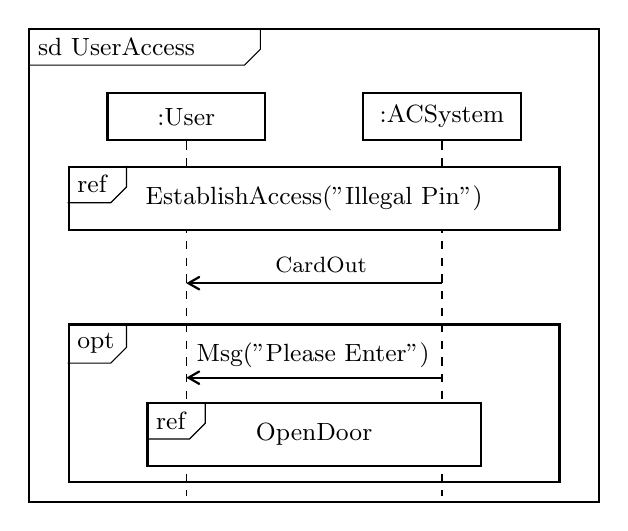
\begin{tikzpicture}
    \tikzstyle{Box}=[align=center, text centered,
    rectangle, draw, thick]
    \tikzstyle{Arrow}=[->, >=angle 60, thick]
    %\draw [help lines, step=0.5cm] (-4,-4) grid (4,4) ;
    \node (Body) [minimum height=6cm, text width=7cm, Box] {};
    \node (Name) [below = 0cm of Body.north west, anchor=north west, 
      text width=2.5cm, rectangle, font=\small] {sd UserAccess};
    \draw (Name.south west) -- (Name.south east) --++(+0.2cm,+0.2cm) --([xshift=+0.2cm]Name.north east) ;

    \node (Aux0) [below = 1.0cm of Body.north, rectangle] {} ;
    \node (Obj1) [left = 1.5cm of Aux0, Box, minimum width=2cm, minimum height=0.6cm, font=\small,anchor=center] {:User} ;
    \draw [dashed] (Obj1.south) -- ++(0, -4.5cm) ;

    \node (Obj2) [right = 1.5cm of Aux0, Box, minimum width=2cm, minimum height=0.6cm,  font=\small,anchor=center] {:ACSystem} ;
    \draw [dashed] (Obj2.south) -- ++(0, -4.5cm) ;

    \node (Ref1Body) [below = 0.5cm of Aux0, minimum height=0.8cm, text width=6cm, Box, font=\small, fill=white ] {EstablishAccess("Illegal Pin")};
    \node (Ref1Name) [below = 0cm of Ref1Body.north west, anchor=north west, 
      text width=0.3cm, rectangle, font=\small] {ref};
    \draw (Ref1Name.south west) -- (Ref1Name.south east) --++(+0.2cm,+0.2cm) --([xshift=+0.2cm]Ref1Name.north east) ;

    \draw [Arrow] ([yshift=-1.8cm] Obj2.south)--([yshift=-1.8cm]Obj1.south) node[anchor=south west, xshift=1.0cm, font=\footnotesize] {CardOut};

    \node (OptBody) [below = 2.5cm of Aux0, minimum height=2.0cm, text width=6cm, Box,] {};
    \node (OptName) [below = 0cm of OptBody.north west, anchor=north west, 
      text width=0.3cm, rectangle, font=\small] {opt};
    \draw (OptName.south west) -- (OptName.south east) --++(+0.2cm,+0.2cm) --([xshift=+0.2cm]OptName.north east) ;

    \draw [Arrow] ([yshift=-3.0cm] Obj2.south)--([yshift=-3.0cm]Obj1.south) node[anchor=south west, font=\small] {Msg("Please Enter")};

    \node (Ref2Body) [below = 3.5cm of Aux0, minimum height=0.8cm, text width=4cm, Box, font=\small, fill=white ] {OpenDoor};
    \node (Ref2Name) [below = 0cm of Ref2Body.north west, anchor=north west, 
      text width=0.3cm, rectangle, font=\small] {ref};
    \draw (Ref2Name.south west) -- (Ref2Name.south east) --++(+0.2cm,+0.2cm) --([xshift=+0.2cm]Ref2Name.north east) ;

\end{tikzpicture}
\end{center}
}


\only<4> {

  \centering\begin{tikzpicture} 
    \begin{umlseqdiag}
      \umlobject[class=A]{a} 
      \umlcreatecall [class=B]{a}{b} 
      \begin{umlfragment}[type=alt,label=i>5,inner xsep=2] 
        \begin{umlcall}[op={tata(i, k)}, dt=7, return=2]{a}{b} 
        \end{umlcall}
      \end{umlfragment} 
    \end{umlseqdiag} 
  \end{tikzpicture}
}

 \only<5> {
  \centering\begin{tikzpicture} 
    \begin{umlseqdiag}
      \umlobject[class=A] {a} 
      \umlcreatecall [class=B]{a}{b} 
      \begin{umlfragment}[type=alt, label=i>5,inner xsep=5] 
        \begin{umlcall}[op={tata(i, k)}, dt=7, return=2]{a}{b} 
        \end{umlcall}
        \umlfpart[default] 
        \begin{umlcall}[op={titi(a,k)}, return=4]{a}{b} 
        \end{umlcall}
      \end{umlfragment} 
    \end{umlseqdiag} 
  \end{tikzpicture}
}

\end{frame}


\begin{frame}[t]
  \frametitle{顺序图的几个问题 }
  \begin{columns}[T]

    \column{0.6\hsize} 

  \begin{itemize}
    \item 抽象层次问题 
    \item 局部与全局问题
    \item 时间的表示问题
    \item 文字描述问题
      \begin{itemize}
        \item [] 避免操作细节
        \item [] 简述交互过程
        \item [] 体现外部行为       
        \item [] 围绕系统功能
      \end{itemize}
  \end{itemize}

    \column{0.4\hsize} 
\centering    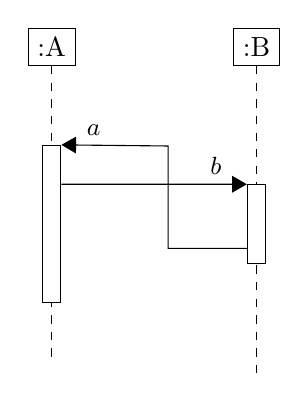
\begin{tikzpicture}
    \node (Obj1) [text centered, rectangle, draw] {:A} ;
    \draw [dashed] (Obj1.south) -- (0, -4cm) ;
    \node (O1) [below = 1.0cm of Obj1, minimum width=0.2cm, minimum
      height=2.0cm, rectangle,
    draw, fill=white] {} ;

    \node (Obj2) [right = 2.0cm of Obj1, text centered, rectangle, draw] {:B} ;
    \draw [dashed] (Obj2.south) -- +(0, -4cm) ;
    \node (O2) [below = 1.5cm of Obj2, minimum width=0.2cm, minimum
      height=1.0cm, rectangle,
    draw, fill=white] {} ;

    \draw [->, >= triangle 60] ([yshift=-0.5cm]O1.north east) --
    (O2.north west) node [font=\small, anchor = south east,
    xshift=-0.2cm] {$b$} ;

    \draw [->, >= triangle 60] ([yshift=+0.2cm]O2.south west) --
    ++(-1cm, 0) -- ++ (0, 1.3cm) -- (O1.north east) node [font=\small,
    anchor = south west, xshift=0.2cm]{$a$} ;
    \end{tikzpicture}

    \centering{例:递归问题 }
  \end{columns}
\end{frame}

\begin{frame}
  \frametitle{如何建立顺序图}
  \begin{itemize}
    \item 决定建立哪些顺序图。基本以用况为单位,但是不绝对 \\
      \quad 简单的用况不必用顺序图描述 \\
      \quad 系统内部的功能也可以用顺序图描述

    \item 确定参加交互的对象和参与者 \\
      \quad 确定参加交互的参与者  \\
      \quad 找出与参与者直接交互的对象  \\
      \quad 以消息为线索,找出与交互有关的全部对象 

    \item 绘制顺序图
  \end{itemize}
\end{frame}

\section{活动图}

\begin{frame}
  \frametitle{活动图}
  \begin{block}{活动图(activity diagram)}
  是一种描述系统行为的图,它把一项行为表示成一个可以由计算机、人或
  者其他执行者执行的活动,通过给出活动中的各个动作以及动作之间的转移关系
  来描述系统的行为
  \end{block}
  活动图起源于流程图(flow chart),同时借鉴了工作流、Petri网等领域的若
  干概念,使其表达能力比流程图更强,应用范围也更宽
\end{frame}

\begin{frame}
  \frametitle{主要概念}
  \begin{block}{活动(activity)}
    是由一系列动作构成的,是对一项系统行为的描述,它不是活
  动图的模型元素,而是一个整体概念,对应着整个活动图
\end{block}
\begin{block} {动作(action)}
  是活动的基本构成单位,被看作一种原子的构造成分 \\
  如果要展开一个动作内部的细节,则: \\
  \quad \textcolor{blue}{UML1}: 定义为“子活动” \\
  \quad \textcolor{blue}{UML2}: 定义为“调用行为”动作
\end{block}

\end{frame}

\begin{frame}
  \frametitle{表示法}
  活动图由\textcolor{blue}{结点(node)}和\textcolor{blue}{边(edge)}两种基本元素构成 \\
  \textcolor{blue}{结点}:动作、判断、合并、分岔、汇合、起点、结束 \\
  \textcolor{blue}{活动边}:控制流和对象流 \\[3ex]
  \begin{tikzpicture}
  \tikzstyle{Action}=[rectangle, rounded corners, draw, thick]
  \tikzstyle{Obj}=[rectangle, draw, thick]
  \node (Action1) [Action] {动作名称1} ;
  \node (Action2) [Action, right = of Action1] {动作名称2 *} ;
  \draw [->, >= angle 60, thick] (Action1) -- (Action2)  ;

  \node (Action3) [Action, below = 0.5cm of Action1] {动作名称3} ;
  \node (Obj1) [Obj, right = of Action3] {对象名称} ;
  \node (Action4) [Action, right = of Obj1] {动作名称4} ;
  \draw [->, >= angle 60, thick] (Action3) -- (Obj1) ;
  \draw [->, >= angle 60, thick] (Obj1) -- (Action4) ;
\end{tikzpicture}
\end{frame}

\begin{frame}
  \frametitle{判断与合并}
  \only<1> {
  \textcolor{blue}{判断(decision)}:控制结点。表示执行到这一点时将判断是否满足某些条件,以决定从不
  同的分支选择下一个动作 \\[2ex]

    \resizebox{!}{2.5cm} {
  \begin{tikzpicture}
    %\umlstatedecision[name=decision]
    \path[draw,thick] (1,0)--(0,1)--(-1,0)--(0,-1)--cycle ;
    \draw [->, >=angle 60, very thick] (0,2)--(0,1) ;
    \draw [->, >=angle 60, very thick] (1,0) node [anchor=south
    west, font=\Large]{[else]} --++(+2,0)--++(0,-1.5) ;
    \draw [->, >=angle 60, very thick] (-1,0)node [anchor=south
    east, font=\Large]{[条件]}--++(-2,0)--++(0,-1.5) ;
  \end{tikzpicture}
  }
  \qquad\resizebox{!}{3cm} {
  \begin{tikzpicture}
    %\draw [help lines, step=0.5cm] (-3,-3) grid (3,3) ;
    \tikzstyle{Line} = [->, >=angle 60, very thick]
    \path[draw,thick] (1,0)--(0,1)--(-1,0)--(0,-1)--cycle ;
    \draw [Line] (0,2)--(0,1) ;
    \draw [Line] (1,0) node [anchor=south west, font=\Large]
      {[else]} --++(+2,0) ;
    \draw [Line] (-1,0) node [anchor=south east, font=\Large]
     {[条件1]}--++(-2,0) ;
    \draw [Line] (-0.5,-0.5) --++(-2.5,-1)node [anchor=north west, font=\Large]
     {[条件2]} ;
    \draw [Line] (0.5,-0.5) --++(2.5,-1)node [anchor=north east, font=\Large]
     {[条件n]} ;
  \end{tikzpicture}
  }
}

\only<2-> {
    \textcolor{blue}{合并(merge)}:控制结点。表示把多个分支合并到一起
    \\[2ex]

 \resizebox{4cm}{!} {
  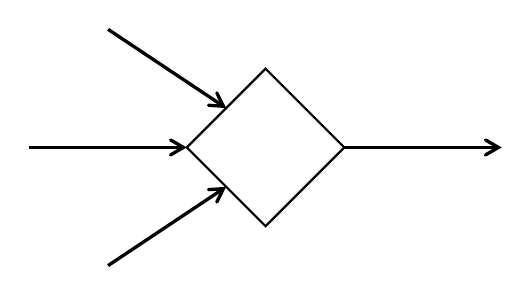
\begin{tikzpicture}
    %\draw [help lines, step=0.5cm] (-3,-3) grid (3,3) ;
    \tikzstyle{Line} = [->, >=angle 60, very thick]
    \path[draw,thick] (1,0)--(0,1)--(-1,0)--(0,-1)--cycle ;
    \draw [Line] (1,0) --(3,0) ;
    \draw [Line] (-2,1.5) --(-0.5,0.5) ;
    \draw [Line] (-3,0) --(-1,0) ;
    \draw [Line] (-2,-1.5) --(-0.5,-0.5) ;
  \end{tikzpicture}
  }
 \qquad\resizebox{4cm}{!} {
  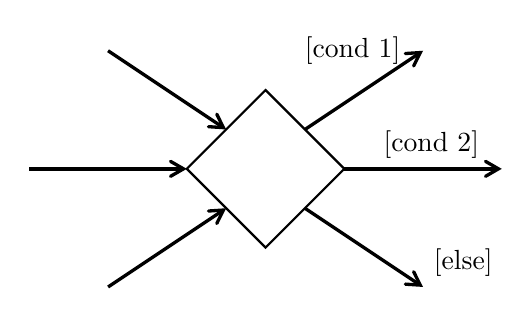
\begin{tikzpicture}
    %\draw [help lines, step=0.5cm] (-3,-3) grid (3,3) ;
    \tikzstyle{Line} = [->, >=angle 60, very thick]
    \path[draw,thick] (1,0)--(0,1)--(-1,0)--(0,-1)--cycle ;
    \draw [Line] (1,0) --(3,0)node[anchor=south east, xshift=-1ex]{[cond 2]} ;
    \draw [Line] (-2,1.5) --(-0.5,0.5) ;
    \draw [Line] (-3,0) --(-1,0) ;
    \draw [Line] (-2,-1.5) --(-0.5,-0.5) ;

    \draw [Line] (0.5,0.5) --(2,1.5)node[anchor= east, xshift=-1ex]{[cond 1]} ;
    \draw [Line] (0.5,-0.5) --(2,-1.5)node[anchor=south west]{[else]} ;
  \end{tikzpicture}
  }
}

  \onslide<3> {
  \textcolor{red}{讨论}:判断与合并结点是成对出现的吗?
  }
\end{frame}

\begin{frame}
  \frametitle{分叉与汇合:用来表示并发行为的控制结点}
  \textcolor{blue} {分岔(fork)}:表示一旦前面的动作结束而流入这个结点,
  它的每个流出边所指的动作都可以执行 \\
  \textcolor{blue} {汇合(join)}:表示汇合点之前有多个控制流在汇合点上
  需要取得同步,并汇合为一个控制流 \\[2ex]

\resizebox{!}{1.5cm} {
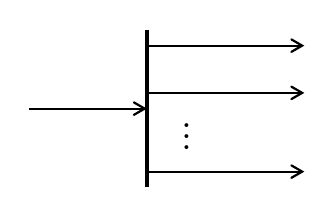
\begin{tikzpicture}
  %\draw [help lines, step=0.5cm] (-1.5, -1) grid (2, 1) ;
  \draw [ultra thick] (0, -1) -- (0, 1) ;
  \draw [->, >=angle 60, thick] (-1.5,0) -- (0, 0) ;
  \draw [->, >=angle 60, thick] (0,0.8) -- (2, 0.8) ;
  \draw [->, >=angle 60, thick] (0,0.2) -- (2, 0.2) ;
  \draw [->, >=angle 60, thick] (0,-0.8) node [anchor=south west,
  xshift=2ex, yshift=1ex, font=\Large]{\vdots} -- (2, -0.8) ;
\end{tikzpicture}
}
\quad\resizebox{!}{1.5cm} {
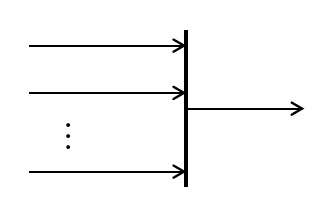
\begin{tikzpicture}
  %\draw [help lines, step=0.5cm] (-2, -1) grid (1.5, 1) ;
  \draw [ultra thick] (0, -1) -- (0, 1) ;
  \draw [->, >=angle 60, thick] (0,0) -- (1.5, 0) ;
  \draw [->, >=angle 60, thick] (-2,0.8) -- (0, 0.8) ;
  \draw [->, >=angle 60, thick] (-2,0.2) -- (0, 0.2) ;
  \draw [->, >=angle 60, thick] (-2,-0.8) node [anchor=south west,
  xshift=2ex, yshift=1ex, font=\Large]{\vdots} -- (0, -0.8) ;
\end{tikzpicture}
}
\quad\resizebox{!}{1.5cm} {
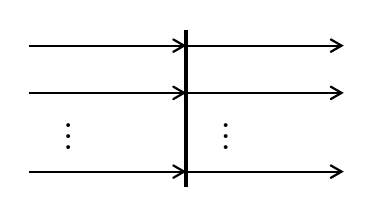
\begin{tikzpicture}
  %\draw [help lines, step=0.5cm] (-2, -1) grid (2, 1) ;
  \draw [ultra thick] (0, -1) -- (0, 1) ;
  \draw [->, >=angle 60, thick] (-2,0.8) -- (0, 0.8) ;
  \draw [->, >=angle 60, thick] (-2,0.2) -- (0, 0.2) ;
  \draw [->, >=angle 60, thick] (-2,-0.8) node [anchor=south west,
  xshift=2ex, yshift=1ex, font=\Large]{\vdots} -- (0, -0.8) ;
  \draw [->, >=angle 60, thick] (0,0.8) -- (2, 0.8) ;
  \draw [->, >=angle 60, thick] (0,0.2) -- (2, 0.2) ;
  \draw [->, >=angle 60, thick] (0,-0.8) node [anchor=south west,
  xshift=2ex, yshift=1ex, font=\Large]{\vdots} -- (2, -0.8) ;
\end{tikzpicture}
}
\pause

\alert{讨论}:分岔与汇合是否必须匹配?

\end{frame}

\begin{frame}
  \frametitle{起点、活动结束和流结束}
  \only<1> {
  \noindent\textcolor{blue}{起点(initial node)}:一个活动图所描述的整个活
  动的开始 \\
  \noindent\textcolor{blue}{活动结束(activity final)}:活动图所描述的整个活
  动到此终结 \\
  \noindent\textcolor{blue}{流结束(flow final)}:表示活动图中一个控制流的终结,
  但并不是整个活动终结 \\[2ex]

  \centering\resizebox{6cm}{!} {
  \begin{tikzpicture}
    \umlstateinitial ;
    \umlstatefinal[x=4] ;
    \umlstateexit[x=8] ;
  \end{tikzpicture} 
  } 
  }

  \only<2> {
  \begin{center}
    \centering\includegraphics[width=1.0\hsize]{flowend.pdf}
  \end{center}
  }

  \only<3> {
  \noindent\begin{center}
    \centering\includegraphics[width=1.1\hsize]{flowend2.pdf}
  \end{center}
  }
\end{frame}


\begin{frame}
  \frametitle{一个活动图的例子}
  \begin{center}
    \centering\includegraphics[width=1.0\hsize]{case1.pdf}
  \end{center}
\end{frame}

\begin{frame}
  \frametitle{泳道}
  \textcolor{blue}{泳道(swim lane)}:
  一种辅助机制,其作用是把活动图中的各个动作划分到与它们的执行者相关的若
  干区域中,从而清晰地表现出不同的执行者分别执行了哪些动作 \\[2ex] 

  \begin{center}
    \centering\includegraphics[width=1.0\hsize]{case1-lane.pdf}
  \end{center}
\end{frame}

\begin{frame}
  \frametitle{发送信号与接受事件动作}
  \textcolor{blue}{接受事件动作(AcceptEventAction)}:如果接受事件动作
  没有输入边,则当活动开始时,它立即开始执行,并且在接受了一个事件后也不
  会终止 \\
  \textcolor{blue}{发送信号动作(SendSignalAction)}:发送异步信号 \\

  \begin{center}
    \centering\includegraphics[width=1.0\hsize]{signal.pdf}
  \end{center}

\end{frame}
  
\begin{frame}
  \frametitle{问题讨论}
  \begin{itemize}
    \item 业务流程和执行过程的差异
    \item 并发描述上的误差 
    \item 对象流问题 
    \item 复杂性问题
  \end{itemize}
  \begin{center}
    \centering\includegraphics[width=1.0\hsize]{case1.pdf}
  \end{center}
\end{frame}

\begin{frame}
  \frametitle{如何使用活动图}
  \begin{itemize}
    \item 描述对象的操作流程
      \begin{itemize}
        \item 未必每个操作,未必十分详细
      \end{itemize}
    \item 描述系统某些局部的行为
      \begin{itemize}
        \item 判断是否真正必要
      \end{itemize}
    \item 描述系统外部可见的行为
      \begin{itemize}
        \item 实际上是描述用况,如果用文字更清楚就用文字
      \end{itemize}
    \item 描述系统的业务流程 
      \begin{itemize}
        \item 注意业务流程和执行过程的差别和并发描述的误差
      \end{itemize}
  \end{itemize}
\end{frame}

\begin{frame}[plain]
  \vspace*{-4ex}
  \begin{center}
    \centering\includegraphics[height=1.00\textheight]{pc.pdf}
  \end{center}
\end{frame}

\section{状态机图}

\begin{frame}
  \frametitle{状态机图}
  \only<1> {
  \begin{block}{状态机图(state machine diagram)}
    是一种描绘系统中的对象(或者其他实体)在其生命期内所经历的
    各种状态,状态之间的转移,发生转移的动因、条件及活动的模型图 \\
  \end{block}

    别称:\textcolor{blue}{状态图(state chart)}、
    \textcolor{blue}{状态转移图(state transition diagram,STD)} \\

    行为状态机与协议状态机
  }

  \only<2> {
    \begin{block}{状态建模}
      通过分析系统(或其局部)所经历的状态和状态之间的转移,用状
    态、转移等概念来建立系统模型 \\
    在某些领域可以作为一种独立的建模方法,
    在面向对象建模中可以起到一种辅助作用
  \end{block}

  \textcolor{blue}{长处}:对状态复杂多变,并且在不同状态下呈现不同行为的对象,通过状态建
    模将有助于准确地认识和描述对象的行为  \\

    \textcolor{blue}{局限性}:一个状态机图通常只适合描述系统中一个或少数几个对象的状态及其
    转移情况,很难用于描述整个系统
  }
  \end{frame}

  \begin{frame}
    \frametitle{状态(state)}
    \only<1> {
    \textcolor{blue}{UML的定义}: 
    \begin{itemize}
      \item “对象生命期中的一种条件或者情形,在此期间它满足某些条件,执行某些
      活动,或者等待某些事件。” \\
    \item “状态是对一种状况的模型表示,在此期间保持了某些(通常是固有的)条
      件。”
    \end{itemize}

      \textcolor{blue}{《对象技术词典》的定义}: \\
      \begin{itemize}
        \item 对象或者类的所有属性的当前值 
        \item 对象或者类的整体行为(例如响应消息)的某些规则所能适应的(对象或类
      的)状况、情况、条件、形式或生存周期阶段
      \end{itemize}
    }
    \only<2> {
    状态机图中的结点,有名字,还可有 \textcolor{blue}{do/action, entry/action, exit/action}等行为\\[2ex]
    \begin{tikzpicture}
      \tikzumlset{fill state=white};

      \tikzstyle{Action}=[rectangle, rounded corners, draw, thick,
      text centered]
      \node (Action1) [Action, minimum height=1cm, text
      width=1.5cm] {state} ;

      \begin{umlstate}[name=state1, x=4] {state1}
      \end{umlstate}

      \begin{umlstate}[name=state2,
                    entry=a,
                    exit=c,
                    do=b, 
                    x=8, y=-1
                    ]{state2}
      \end{umlstate}
    \end{tikzpicture} 
    }
  \end{frame}

\begin{frame}
\frametitle{伪状态(pseudo state)}
伪状态实际上并不是一种状态,只是为了加强状态机图的可视化效果而引入的一些图形符号,是结点(顶点)型的图形成分\\[2ex]
\begin{tikzpicture}
\tikzstyle{Font}=[font=\small]
\umlstateinitial [name=initial ] 
\umlstatefinal [x=2, name=final]
\umlstatejoin [x=4, name=join]
\umlstatedecision [x=6, name=decision]
\umlstateenter[y=-2, name=enter]
\umlstateexit [x=2, y=-2, name=exit]
\umlstateend [x=4, y=-2, name=end]
\umlstatehistory [x=6,y=-2, name=hist]
\umlstatedeephistory [x=8, y=-2, name=deephist]
\node [below = 0.2cm of initial, Font] {initial} ;
\node [below = 0.2cm of final, Font] {final} ;
\node [below = 0.4cm of join, Font] {junction} ;
\node [below = 0.4cm of decision, Font] {decision} ;
\node [below = 0.2cm of enter, Font] {enter} ;
\node [below = 0.2cm of exit, Font] {exit} ;
\node [below = 0.2cm of end, Font] {end} ;
\node [below = 0.2cm of hist, Font] {history} ;
\node [below = 0.2cm of deephist, Font] {deep history} ;
\end{tikzpicture}
\end{frame}

\begin{frame}
\frametitle{组合状态(composite state)}
由若干状态组织在一起所形成的状态称为\textcolor{blue}{组合状态} \\
包含在组合状态内部的状态称为\textcolor{blue}{子状态},内部不包含其他状态
的状态称为\textcolor{blue}{简单状态} \\[2ex]

\begin{tikzpicture}
\tikzumlset{fill state=white};
\begin{umlstate}[name=state ]{state} 
\umlbasicstate[name=substate1]{sub state1} 
\umlbasicstate[x=4, name=substate2]{sub state2}
\umltrans[anchor1=-20, anchor2=200]{substate1}{substate2}
\umltrans[anchor1=160, anchor2=20]{substate2}{substate1}
\end{umlstate} 
\end{tikzpicture}

组合状态的作用:使模型更清晰、便于复用、简化图的绘制

\end{frame}


\begin{frame}
  \frametitle{转移(transition) }

    \textcolor{blue}{转移}:状态机图中的边,描述了从一个状态到另一个状态的转变\\
    可以有触发器(trigger,UML1中称为事件event),监护约束(guard)或行为表达式(behaviour-expression) \\[3ex]

    \begin{tikzpicture}
      \tikzumlset{fill state=white};

      \begin{umlstate}[name=state1] {state1}
      \end{umlstate}

      \begin{umlstate}[name=state2, x=6] {state2}
      \end{umlstate}

      \umlVHVtrans[arm1=-2cm, arg=触发器[监护约束]/行为表达式, pos=1.5] {state1}{state2}   

      \umltrans[recursive=-20|20|1cm, arg=$a$ , pos=1.5, recursive direction=right to right ]{state2}{state2}

    \end{tikzpicture} 
\end{frame}

\begin{frame}
\frametitle{ATM示例}

\only<1> {
\begin{tikzpicture}
\tikzumlset{fill state=white};

\begin{umlstate}[name=Atm]{客户使用ATM机}
\umlstateinitial[name=Ainit]
\umlbasicstate[y=-2.5, name=Authen]{认证}
\umlbasicstate[x=6, y=-2.5, name=Withdraw]{取钱}
\umltrans{Ainit}{Authen}
\umltrans[arg={检查密码}, pos=0.5]{Authen}{Withdraw}

\end{umlstate}
\end{tikzpicture}
}

\only<2> {
\begin{tikzpicture}
\tikzumlset{fill state=white};

\begin{umlstate}[name=Atm]{客户使用ATM机}
\umlstateinitial[name=Ainit]
\umlbasicstate[y=-2.5, name=Authen]{认证}
\umlbasicstate[x=7, y=-2.5, name=Withdraw]{取钱}
\umltrans{Ainit}{Authen}
\umltrans[arg={检查密码$[$正确$]$}, pos=0.5]{Authen}{Withdraw}
\umltrans[recursive=-20|-60|1.5cm, recursive direction=right to bottom, 
  arg={检查密码$[$错误$]$}, pos=1.5]{Authen}{Authen}

\end{umlstate}
\end{tikzpicture}
}

\only<3> {
\begin{tikzpicture}
\tikzumlset{fill state=white};

\begin{umlstate}[name=Atm]{客户使用ATM机}
\umlstateinitial[name=Ainit]
\umlbasicstate[y=-2.5, name=Authen]{认证}
\umlbasicstate[x=6, y=-2.5, name=Withdraw]{取钱}
\umltrans{Ainit}{Authen}
\umltrans[arg={检查密码$[$正确$]$}, pos=0.5]{Authen}{Withdraw}
\umltrans[recursive=-20|-60|1.5cm, recursive direction=right to bottom, 
  arg={检查密码$[$错误$]/$尝试次数加1}, pos=1.9]{Authen}{Authen}

\umlbasicstate[x=6, y=-2.5, name=Withdraw]{取钱}

\end{umlstate}
\end{tikzpicture}
}

\only<4> {
  \resizebox{1.0\hsize}{!} {
\begin{tikzpicture}
\tikzumlset{fill state=white};

\begin{umlstate}[name=Atm]{客户使用ATM机}
\umlstateinitial[name=Ainit]
\umlbasicstate[y=-2.2, name=Authen]{认证}
\umlbasicstate[x=9, y=-2.2, name=Withdraw]{取钱}
\umltrans{Ainit}{Authen}
\umltrans[arg={检查密码$[$正确$]$}, pos=0.5]{Authen}{Withdraw}
\umltrans[recursive=-20|-60|1.4cm, recursive direction=right to bottom, 
  arg={$\text{检查密码}[\text{错误且}ErrCnt<Limit]/ErrCnt+1$}, pos=1.9]{Authen}{Authen}

\umlbasicstate[y=-5.5, name=Reject]{拒绝}

\umltrans[arg={$\text{检查密码}[\text{错误且}ErrCnt>=Limit]/\text{通知认
证失败}$}]
{Authen}{Reject}

\end{umlstate}
\end{tikzpicture}
}
}

\only<5> {
  \resizebox{0.9\hsize}{!} {
\begin{tikzpicture}
\tikzumlset{fill state=white};

\begin{umlstate}[name=Atm]{客户使用ATM机}
\umlstateinitial[y=1, name=Ainit]
\begin{umlstate}[y=-3, width=2.5cm, name=Authen, do=CheckPIN, entry=maskScreen,
  exit=unmaskScreen]{认证}
\end{umlstate}
\umlbasicstate[x=8, y=-1.95, name=Withdraw]{取钱}
\umltrans{Ainit}{Authen}
\umltrans[arg={检查密码$[$正确$]$}, pos=0.7]{Authen}{Withdraw}
\umltrans[recursive=-20|-60|1.6cm, recursive direction=right to bottom, 
  arg={$\text{检查密码}[\text{错误且}ErrCnt<Limit]/ErrCnt+1$}, pos=1.9]{Authen}{Authen}

\umlbasicstate[y=-5.5, name=Reject]{拒绝}

\umltrans[arg={$\text{检查密码}[\text{错误且}ErrCnt>=Limit]/\text{通知认
证失败}$}]
{Authen}{Reject}
\end{umlstate}
\end{tikzpicture}
}
}
\end{frame}

\begin{frame}
  \frametitle{深入理解事件}
\noindent  \resizebox{1.0\hsize}{!} {
\begin{tikzpicture}
\tikzumlset{fill state=white};

\begin{umlstate}[name=state1, width=2cm, do=ActDo1, entry=ActEntry1,
  exit=ActExit1]{状态1}
\end{umlstate}
\begin{umlstate}[x=9, name=state2, width=2cm, do=ActDo2, entry=ActEntry2,
  exit=ActExit2]{状态2}
\end{umlstate}
\umltrans[arg={$Ev(Arg)[Guard]/ActTrans(Arg, Arg1)$}, pos=0.5]{state1}{state2}
\end{tikzpicture}
}

\begin{enumerate}
  \item 某处的某个动作产生了一个事件Ev
  \item Ev传播到了当前对象
  \item Ev进入当前对象的事件队列
  \item Ev被从队列中取出,变成当前事件
  \item Ev被处理
\end{enumerate}
\end{frame}

\begin{frame}
  \frametitle{事件处理}
\noindent  \resizebox{1.0\hsize}{!} {
\begin{tikzpicture}
\tikzumlset{fill state=white};

\begin{umlstate}[name=state1, width=2cm, do=ActDo1, entry=ActEntry1,
  exit=ActExit1]{状态1}
\end{umlstate}
\begin{umlstate}[x=9, name=state2, width=2cm, do=ActDo2, entry=ActEntry2,
  exit=ActExit2]{状态2}
\end{umlstate}
\umltrans[arg={$Ev(Arg)[Guard]/ActTrans(Arg, Arg1)$}, pos=0.5]{state1}{state2}
\end{tikzpicture}
}

\begin{enumerate}
  \item 检查$Guard$,如果$false$放弃
  \item 中止 ActDo1
  \item 执行 ActExit1
  \item 执行 ActTrans(Arg, Arg1). 注:同步调用
  \item 执行 ActEntry2
  \item 执行 ActDo2
\end{enumerate}
\end{frame}

\begin{frame}
  \frametitle{事件处理:Completion 事件}
\noindent  \resizebox{1.0\hsize}{!} {
\begin{tikzpicture}
\tikzumlset{fill state=white};

\begin{umlstate}[name=state1, width=2cm, do=ActDo1, entry=ActEntry1,
  exit=ActExit1]{状态1}
\end{umlstate}
\begin{umlstate}[x=9, name=state2, width=2cm, do=ActDo2, entry=ActEntry2,
  exit=ActExit2]{状态2}
\end{umlstate}
\umltrans[arg={$[Guard]/ActTrans(Arg1)$}, pos=0.5]{state1}{state2}
\end{tikzpicture}
}

\begin{enumerate}
  \item 等待直到ActDo1结束(触发completion事件)
  \item 检查$Guard$,如果$false$放弃
  \item 执行 ActExit1
  \item 执行 ActTrans(Arg1)
  \item 执行 ActEntry2
  \item 执行 ActDo2
\end{enumerate}
\end{frame}

\begin{frame}
  \frametitle{事件处理:Change 事件}
\noindent  \resizebox{1.0\hsize}{!} {
\begin{tikzpicture}
\tikzumlset{fill state=white};

\begin{umlstate}[name=state1, width=2cm, do=ActDo1, entry=ActEntry1,
  exit=ActExit1]{状态1}
\end{umlstate}
\begin{umlstate}[x=9, name=state2, width=2cm, do=ActDo2, entry=ActEntry2,
  exit=ActExit2]{状态2}
\end{umlstate}
\umltrans[arg={$when(Guard)/ActTrans(Arg1)$}, pos=0.5]{state1}{state2}
\end{tikzpicture}
}

\begin{enumerate}
  \item 等待直到Guard由$false$变为$true$(触发change事件)
  \item 中止 ActDo1
  \item 执行 ActExit1
  \item 执行 ActTrans(Arg1)
  \item 执行 ActEntry2
  \item 执行 ActDo2
\end{enumerate}
\end{frame}

\begin{frame}
  \frametitle{Completion和Change事件的比较}
  \textcolor{blue}{Activity} \\
  Completion 事件:  ActDo1 执行完成  \\
  Change 事件: 中止ActDo1 \\[2ex]
  \textcolor{blue}{Guard} \\
  Completion 事件: 监护条件只检查一次  \\
  Change 事件: 持续检查监护条件

\end{frame}

\begin{frame}
  \frametitle{区域(region)}
  区域之间的状态是正交的,区域用于表示并发转移 \\[3ex]
  \centering\includegraphics[width=1.0\hsize]{complexstate1.pdf}
\end{frame}

\begin{frame}
  \frametitle{历史状态}
  \centering\includegraphics[width=1.0\hsize]{complexstate2.pdf}
\end{frame}

\begin{frame}
  \frametitle{如何使用状态机图:作为辅助模型}
  \begin{itemize}
    \item 仅对状态对行为影响复杂的对象建立状态机图
    \item 使用主要概念:状态、转移、组合状态、伪状态
    \item 识别对行为有不同影响的对象状态,达到如下效果:
      \begin{itemize}
        \item 在不同的状态下对象将呈现不同的行为规则
        \item 同一种状态下对象的行为规则始终一致
      \end{itemize}
    \item 认识和描述转移:触发器、监护约束、行为表达式
    \item 为类图提供有用的信息:状态——属性;转移——操作
  \end{itemize}

\end{frame}

\section{构件图}

\begin{frame}
  \frametitle{构件图(component diagram)}
  \begin{block}{构件图}
    是一种表示构件的组织结构和相互关系的图,用于表达在实现时如何将
    系统元素组织成构件,从而支持以构件为单位进行软件制品的实现和发布
  \end{block}

    UML1的构件图没有太多地反映当时构件技术的发展,它只是着眼于把软件的逻
    辑蓝图转化为计算机世界中的事物 \\

     UML2为构件图增添了许多内容,能够表示构件技术领域的大部分常用的概念

\end{frame}

\begin{frame}
  \frametitle{主要概念}
  \only<1> {
  \begin{block}{构件(component)}
    OMG:“一个构件表示系统中一个模块部件,它封装了它的内容,而
    其表现形式在其环境中是\alert{可替换}的。”
  \end{block}

  通常:可复用构件的简称,特指按某种构件标准设计,并可在多个系统中重复使用的软
  件构造块。构件被认为是自治和独立的。
  }
 \only<2> {
  \begin{block}{接口(interface)}
    UML2:“接口是一种类目,它表示对一组紧凑的公共特征和职责的声明。一个接口说
    明了一个合约;实现接口的任何类目的实例必须履行这个合约。” 
  \end{block}
  供接口(provided interface): 实现的接口 \\
  需接口(required interface): 使用的接口
  }
 \only<3> {
  \begin{block}{端口(port)}
    UML2:“类目的一个特征,指出类目与外部环境之间或者与内部的部件之间的一个明
    显的交互点。” 
  \end{block}
    向内,可以连接到与外部交互的内部成分,称为供端口(provided port) \\
    向外,连接到供接口或者需接口,称为需端口(required port)
  }
  \only<4> {
        实现(realization)和使用(use)是构件和接口之间的两种关系 
        \begin{itemize}
          \item 构件与供接口之间为\textcolor{blue}{实现关系},称为
        \textcolor{blue}{接口实现}(InterfaceRealization)
      \item 构件与需接口之间为\textcolor{blue}{使用关系} 
    \end{itemize}

        \textcolor{blue}{构件实现}(ComponentRealization):构件中的类实现了该构件依据其接
        口所提供的合约
  }
  \only<5> {
    \begin{block}{委派连接件(delegation connector)}
      是从构件的端口连接到构件内部
    成分的连接件,它“把构件外部的一个合约(由它的端口说明)链接到由构件
    中的部件对这个行为的内部实现。”  
  \end{block}
  \begin{block}{组装连接件(assembly connector)}
    是两个构件之间的连接件,
      它表明一个构件提供了另一个构件所需要的服务。 \\
      一个供接口和一个需接口之间的衔接就表示一个组装连接件
    \end{block}
  }
\end{frame}

\begin{frame}
  \frametitle{表示法}
  \only<1> {
    用 <<component>> 或者 
    \resizebox{!}{0.5cm}{
  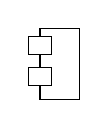
\begin{tikzpicture}
    \node (N1) [rectangle, draw, minimum width=0.5cm, minimum height=0.9cm]
    {} ;
    \node (N2) [rectangle, draw, minimum width=0.3cm, minimum
      height=0.15cm, below = 0.1cm of N1.north, xshift=-0.25cm, fill=white] {} ;
    \node [rectangle, draw, minimum width=0.3cm, minimum height=0.15cm,
    below = 0.15cm of N2, fill=white] {} ;
  \end{tikzpicture}
} 表示构件, 二者等价 \\[2ex]

  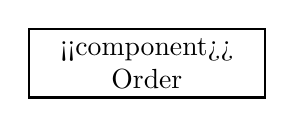
\begin{tikzpicture}
    \node [rectangle, draw, thick,align=center, minimum width=3cm] {<<component>> \\ Order} ;
  \end{tikzpicture}%
  \quad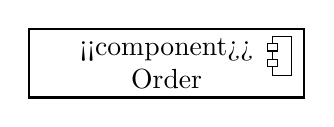
\begin{tikzpicture}
    \node (C) [rectangle, draw, thick,align=center, minimum width=3.5cm] {<<component>> \\ Order} ;
    \node (N1) [rectangle, draw, minimum width=0.2cm, minimum
    height=0.5cm, below=0.10cm of C.north east, xshift=-0.3cm] {} ;
    \node (N2) [rectangle, draw, minimum width=0.3cm, scale=0.4, minimum
      height=0.1cm, below = 0.1cm of N1.north, xshift=-0.3cm, fill=white] {} ;
    \node [rectangle, draw, minimum width=0.3cm, minimum height=0.1cm,
    below = 0.1cm of N2, fill=white, scale=0.4] {} ;
  \end{tikzpicture}

  \vspace*{3ex}
  \centering \begin{tikzpicture}
    \tikzumlset{fill component=white} ;
    \umlbasiccomponent{Order}
    \umlrequiredinterface[interface=\space, distance=2cm]{Order} 
    \umlprovidedinterface [interface=\space, distance=2cm]{Order}
  \end{tikzpicture}
}

  \only<2> {
    \begin{columns}[t]
      \column{0.5\hsize}
    外部视图或黑盒视图 \\[1ex]
    \begin{tikzpicture}
    \node (C) [rectangle, draw, thick,align=center, minimum width=4.5cm] {<<component>> \\ Order} ;
    \node[rectangle,draw, thick, align=left, minimum width=4.5cm,
      below=0cm of C.south, anchor=north] {
      «provided interfaces»  \\
      \hspace*{2ex}OrderEntry \\
      \hspace*{2ex}Billing \\
      «required interfaces»  \\
      \hspace*{2ex}Invoice \\
      \hspace*{4ex}create (\dots) \\
      \hspace*{4ex}registerPayment (\dots)
    };
    \end{tikzpicture}%

    \column{0.5\hsize}
    内部视图或白盒视图 \\[1ex]
    \begin{tikzpicture}
      \tikzstyle{Node}=[rectangle, draw, thick, minimum width=4.5cm]
      \baselineskip=14pt
    \node (C) [align=center, Node] {
      <<component>> \\
      Order} ;
    \node (I) [align=left, Node, below=0cm of C.south, anchor=north] {
      \begin{minipage}{4cm}
      \baselineskip=14pt
      «provided interfaces»\\
      \hspace*{2ex}OrderEntry \\
      \hspace*{2ex}AccountPayable \\
      «required interfaces»  \\
      \hspace*{2ex}Person 
    \end{minipage}
    };
    \node (R) [align=left, Node, below=0cm of I.south, anchor=north] {
      \begin{minipage}{4cm}
      \baselineskip=14pt
      «realizations»  \\
      \hspace*{2ex}OrderHeader \\
      \hspace*{2ex}AccountLineItem 
    \end{minipage}
    };
    \node (A) [align=left, Node, below=0cm of R.south, anchor=north] {
      \begin{minipage}{4cm}
      \baselineskip=14pt
      «artifacts»  \\
      \hspace*{2ex}order.jar
    \end{minipage}
    };
    \end{tikzpicture}
  \end{columns}
  }
  \only<3> {
    显示构件内部成分 \\[2ex]
  \centering\begin{tikzpicture}
    \tikzumlset{fill component=white, fill class=white}
    \begin{umlcomponent}[x=0,y=0]{A} 
      \umlemptyclass{OrderHeader}
      \umlemptyclass[y=-3]{LineItem}
      \umlcompo[mult1=1, mult2=*, arg1=Order, arg2=item]{OrderHeader}{LineItem}
    \end{umlcomponent}
    \umlrequiredinterface[interface=Person, distance=3cm]{A} 
    \umlprovidedinterface [interface=OrderEntry]{A}
  \end{tikzpicture}
}

  \only<4> {
    组装连接件 \\[2ex]
  \centering\begin{tikzpicture}
    \tikzumlset{fill component=white}
    \umlbasiccomponent{A}
    \umlbasiccomponent[x=4, y=-3]{B}
    \umlHVHassemblyconnector [interface=AB1, arm1=6cm, last arm]{A}{B}
    \umlHVHassemblyconnector [interface=AB2]{A}{B}
    \umlVHassemblyconnector [interface=AB3, first arm]{A}{B}
  \end{tikzpicture}
  }

  \only<5> {
    委派连接件 \\[2ex]
    \centering\begin{tikzpicture}
      \tikzumlset{fill component=white, fill port=white}
      \begin{umlcomponent}{A}
      \umlbasiccomponent{B} 
      \umlbasiccomponent[y=-2.8]{C}

      \umlprovidedinterface[interface=Bpi , distance=2cm, padding=2cm]{B} 
      \umlprovidedinterface[interface=Cpi , distance=2cm, padding=2cm]{C}
      \end{umlcomponent}

      \umldelegateconnector{A-west-port}{B-west-interface}
      \umlHVHdelegateconnector[pos stereo=1.5]{A-west-port}{C-west-interface}

      \umlport{A}{west}
    \end{tikzpicture}
  }

  \only<6> {
    构件实现 \\[2ex]
    \centering\begin{tikzpicture}
      \tikzumlset{fill component=white, fill class=white}
      \umlbasiccomponent{Order} 
      \umlemptyclass[x=-2, y=-3]{OrderHeader}
      \umlemptyclass[x=3, y=-3]{LineItem}
      \umlreal{LineItem}{Order}
      \umlreal{OrderHeader}{Order}
    \end{tikzpicture}
  }

  \only<7> {
    接口实现 \\[2ex]
    \centering\begin{tikzpicture}
      \tikzumlset{fill component=white, fill class=white}
      \umlbasiccomponent{Order} 
      \umlclass[type=interface,
      x=-4]{OrderEntry}{}{Create() \\ ValidateDetails() \\
      AddOrderline()}
      \umlclass[type=interface, x=4]{Person}{}{FindbyName() \\
      Create() \\GetDetails()}
      \umlreal{Order}{OrderEntry}
      \umldep{Order}{Person}
    \end{tikzpicture}
  }

  \only<8> {
    构件依赖 \\[2ex]
    \centering
    \resizebox{!}{4.5cm}{\begin{tikzpicture}
      \tikzumlset{fill component=white, fill class=white}
      \umlbasiccomponent{Order} 
      \umlbasiccomponent[x=3]{Customer} 
      \umlbasiccomponent[y=-3]{Product} 
      \umldep{Order}{Product}
      \umldep{Order}{Customer}
    \end{tikzpicture}}%
    \quad\resizebox{!}{4.5cm}{
    \begin{tikzpicture}
      \tikzumlset{fill component=white, fill class=white}
      \umlbasiccomponent{Order} 
      \umlbasiccomponent[x=4]{Customer} 
      \umlbasiccomponent[y=-4]{Product} 
      \umlassemblyconnector[anchors=270 and 90, interface=OrderableItem]{Order}{Product}
      \umlassemblyconnector[interface=Person]{Order}{Customer}
    \end{tikzpicture} }
  }
\end{frame}

\begin{frame}
  \frametitle{端口与连接件}
\resizebox{\hsize}{!}{
\begin{tikzpicture}
\tikzumlset{fill component=white, fill port=white}
\begin{umlcomponent}{A}
  \umlbasiccomponent[width=4ex]{B}
\umlbasiccomponent[width=4ex,x=2]{C}

\umlrequiredinterface[interface=CI, distance=1.5cm, padding=0cm]{C}
\umlprovidedinterface[interface=BI, with port, distance=1.5cm,
padding=1.5cm]{B}
\end{umlcomponent}
\umlbasiccomponent[width=4ex, x=-6]{D}
\umlbasiccomponent[x=3,y=-4, width=4ex]{E}
\umlbasiccomponent[x=-1, y=-4, width=4ex]{F}
\umlbasiccomponent[x=-6,y=-2.5, width=4ex]{G}
\umlbasiccomponent[x=-6,y=-4.5, width=4ex]{H}

\umlassemblyconnector[interface=DA, with port, name=toto]{D}{A}
\umldelegateconnector{A-west-port}{B-west-interface}
\umlVHVassemblyconnector[interface=AE, with port]{A}{E}
\umlassemblyconnector[interface=EF, with port]{E}{F}
\umlHVHassemblyconnector[interface=GHF, with port, arm2=-2cm, last arm]{G}{F}
\umlHVHassemblyconnector[with port, arm2=-2cm, last arm]{H}{F}
\end{tikzpicture}
}
\end{frame}

\begin{frame}
  \frametitle{如何使用构件图}
  \begin{itemize}
    \item 用构件的图形符号表示每个构件
      \begin{itemize}
        \item UML提供了多种构件表示方式,可以有选择地采用
        \item 建模工具应支持多种表示方式之间的切换
      \end{itemize}

    \item 定义构件的接口 
      \begin{itemize}
        \item 考察构件中各个类的操作,发现构件的供接口和需接口
      \end{itemize}

    \item 定义连接件 
      \begin{itemize}
        \item 考察构件之间的关系,定义组装连接件
        \item 根据需要为构件接口和内部成分定义委派连接件 
      \end{itemize}
  \end{itemize}
\end{frame}

\section{部署图}

\begin{frame}
  \frametitle{部署图}
  UML1的定义:“一种显示运行时的处理结点以及在其上生存的构件、进程及对象
  配置的图。”  \\[2ex]

  UML2的定义:“部署图展示了\textcolor{blue}{制品}在\textcolor{blue}{结点
  }上根据它们之间部署的定义所做的\textcolor{blue}{定位}
  。”\\[2ex]

  变化:部署在结点上的软件成分不再是构件,而是\alert{制品}
\end{frame}

\begin{frame}
  \frametitle{主要概念}
  \only<1> {
  \begin{block}{结点(node)}
    表示一个硬件设备或执行环境,即被开发的软件制品将要部署于
  其上的宿主设备或环境  
\end{block}

  \begin{block}{制品(artifact)}
    “制品是对软件开发过程中或系统的部署与操作中所使用或产
  生的信息的物理块的说明。制品的例子包括模型文件、源文件、草稿、二进制可
  执行文件、数据库表、开发交付项、或者字处理的文档、邮件消息等。”  
\end{block}
  }

  \only<2> {
    \begin{block}{执行环境(ExecutionEnvironment)}
      “执行环境是一个结点,它为以可执行制品
  的形式部署于其上的各类构件提供了一个执行环境。”  
\end{block}

  \begin{block}{各种关系} 
  部署(deploy)依赖 \\
  制品之间的依赖 \\
  结点之间的关联
  \end{block}
  }
\end{frame}

\begin{frame}[label=current]
  \frametitle{表示法}
  \only<1> {
  %\begin{center}
    %\centering\includegraphics[width=0.5\hsize]{dep-manifest.pdf}
  %\end{center}
    \begin{tikzpicture}
      \tikzumlset{fill component=white, fill class=white}
      \umlbasiccomponent{Order}
      \umlprovidedinterface{Order}

      \node [rectangle, draw, text width=3cm, below=2.5 of
      Order, align=center, inner sep=2ex] (Jar) {<<artifact>> \\ Order.jar} ;

      \draw ([xshift=-2ex, yshift=-3ex]Jar.north east) -- ++(6pt, 0)
        -- ++(0, 8pt) -- ++(-2pt, 0) -- ++ (0, 2pt) ;

      \draw ([xshift=-2ex, yshift=-3ex]Jar.north east) -- ++(0, 10pt)
        -- ++(4pt, 0) -- ++(2pt, -2pt) ;

        \umldep[stereo=manifest]{Jar}{Order}
        
    \end{tikzpicture}
  }
  \only<2> {
  %\begin{center}
    %\centering\includegraphics[width=0.8\hsize]{dep-loc1.pdf}
%
    %\centering\includegraphics[height=3cm]{dep-loc2.pdf}%
    %\quad\includegraphics[height=3.5cm]{dep-loc3.pdf}

    \centering\begin{tikzpicture}[scale=0.9]
      \node [rectangle, draw, text width=10cm, align=center, minimum
      height=2.4cm] (AppS) {} ;
      \node [below = 0.1 of AppS.north, align=center] {
        \textbf{\uline{:AppServer}}} ;
      \draw ([xshift=-2ex, yshift=-3ex]AppS.north east) -- ++(6pt, 0)
        -- ++(0, 8pt) -- ++(-2pt, 0) -- ++ (0, 2pt) ;
      \draw ([xshift=-2ex, yshift=-3ex]AppS.north east) -- ++(0, 10pt)
        -- ++(4pt, 0) -- ++(2pt, -2pt) ;

      \node [rectangle, draw, text width=3cm, minimum height=1.3cm, 
        align=center] at (-3, -0.3) (Shop) {} ;
      \node [below = 0.1 of Shop.north, align=center] {<<artifact>> \\[-1ex]
        \textbf{\uline{ShoppingCart.ear}}} ;
      \draw ([xshift=-2ex, yshift=-3ex]Shop.north east) -- ++(6pt, 0)
        -- ++(0, 8pt) -- ++(-2pt, 0) -- ++ (0, 2pt) ;
      \draw ([xshift=-2ex, yshift=-3ex]Shop.north east) -- ++(0, 10pt)
        -- ++(4pt, 0) -- ++(2pt, -2pt) ;

      \node [rectangle, draw, text width=3cm, minimum height=1.3cm, 
        align=center, right=2.5 of Shop] (Order) {} ;
      \node [below = 0.1 of Order.north, align=center] {<<artifact>> \\[-1ex]
        \textbf{\uline{Order.ear}}} ;
      \draw ([xshift=-2ex, yshift=-3ex]Order.north east) -- ++(6pt, 0)
        -- ++(0, 8pt) -- ++(-2pt, 0) -- ++ (0, 2pt) ;
      \draw ([xshift=-2ex, yshift=-3ex]Order.north east) -- ++(0, 10pt)
        -- ++(4pt, 0) -- ++(2pt, -2pt) ;

      \draw [-Straight Barb, dashed] (Shop) -- (Order) ;

    \end{tikzpicture}

    \vspace*{2ex}

    \centering\begin{tikzpicture}[scale=0.9]
      \node [rectangle, draw, text width=2.5cm, align=center, minimum
      height=1cm] (AppServer) {} ;
      \node [below = 0.2 of AppServer.north] {\textbf{\uline{:AppServer}}} ;
      \draw (AppServer.north west) -- ++(0.2cm, 0.2cm) -|
      ([xshift=0.2cm, yshift=0.2cm]AppServer.south east) --
      (AppServer.south east);
      \draw (AppServer.north east) -- ([xshift=0.2cm,
      yshift=0.2cm]AppServer.north east) ;

      \node [rectangle, draw, text width=1.5cm, align=center, 
        inner sep=2ex] (Jar1) at (-2, -2.5) {Order.jar} ;
      \draw ([xshift=-2ex, yshift=-3ex]Jar1.north east) -- ++(6pt, 0)
        -- ++(0, 8pt) -- ++(-2pt, 0) -- ++ (0, 2pt) ;
      \draw ([xshift=-2ex, yshift=-3ex]Jar1.north east) -- ++(0, 10pt)
        -- ++(4pt, 0) -- ++(2pt, -2pt) ;
        \draw [-Straight Barb, dashed] (Jar1) -- node [left] {<<deploy>>}
      (AppServer) ;
 
      \node [rectangle, draw, text width=2.8cm, align=center, 
        inner sep=2ex] (Jar2) at (1.5, -2.5) {ShoppingCart.jar} ;
      \draw ([xshift=-2ex, yshift=-3ex]Jar2.north east) -- ++(6pt, 0)
        -- ++(0, 8pt) -- ++(-2pt, 0) -- ++ (0, 2pt) ;
      \draw ([xshift=-2ex, yshift=-3ex]Jar2.north east) -- ++(0, 10pt)
        -- ++(4pt, 0) -- ++(2pt, -2pt) ;
        \draw [-Straight Barb, dashed] (Jar2) -- node [right] {<<deploy>>}
      (AppServer) ;

      \node [rectangle, draw, text width=3cm, align=center, minimum
      height=4.3cm, right= 4.2 of AppServer.north east, anchor=north] (JEE) {} ;
      \draw (JEE.north west) -- ++(0.2cm, 0.2cm) -|
      ([xshift=0.2cm, yshift=0.2cm]JEE.south east) --
      (JEE.south east);
      \draw (JEE.north east) -- ([xshift=0.2cm, yshift=0.2cm]JEE.north east) ;
      \node [below = 0.1 of JEE.north, align=center]
      {\textbf{\uline{:AppServer}}} ;

      \node [below = 0.8 of JEE.north, align=left] {
        Order.jar \\[-2pt] ShoppingCart.jar \\[-2pt] 
        Account.jar \\[-2pt] Product.jar \\[-2pt]
        BackOrder.jar \\[-2pt] Service.jar} ;


 
    \end{tikzpicture}
  }
  \only<3> {
  %\begin{center}
    %\centering\includegraphics[width=1.0\hsize]{dep-desc.pdf}
  %\end{center}
    \centering\begin{tikzpicture}
      \node [rectangle, draw, text width=11cm, align=center, minimum
      height=7cm] (AppServer) {} ;
      \draw (AppServer.north west) -- ++(0.2cm, 0.2cm) -|
      ([xshift=0.2cm, yshift=0.2cm]AppServer.south east) --
      (AppServer.south east);
      \draw (AppServer.north east) -- ([xshift=0.2cm,
      yshift=0.2cm]AppServer.north east) ;
      \node [below = 0.1 of AppServer.north, align=center] {<<device>>
        \\[-1ex] \textbf{\uline{:AppServer}}} ;

      \node [rectangle, draw, text width=10cm, align=center, minimum
      height=5.5cm, below=1.3 of AppServer.north] (Ear) {} ;
      \node [below = 0.1 of Ear.north, align=center] {<<artifact>> \\[-1ex]
        \textbf{\uline{ShoppingApp.ear}}} ;
      \draw ([xshift=-2ex, yshift=-3ex]Ear.north east) -- ++(6pt, 0)
        -- ++(0, 8pt) -- ++(-2pt, 0) -- ++ (0, 2pt) ;
      \draw ([xshift=-2ex, yshift=-3ex]Ear.north east) -- ++(0, 10pt)
        -- ++(4pt, 0) -- ++(2pt, -2pt) ;

      \node [rectangle, draw, text width=3cm, minimum height=1.3cm, 
        align=center] at (-3, 0) (Shop) {} ;
      \node [below = 0.1 of Shop.north, align=center] {<<artifact>> \\[-1ex]
        \textbf{\uline{ShoppingCart.ear}}} ;
      \draw ([xshift=-2ex, yshift=-3ex]Shop.north east) -- ++(6pt, 0)
        -- ++(0, 8pt) -- ++(-2pt, 0) -- ++ (0, 2pt) ;
      \draw ([xshift=-2ex, yshift=-3ex]Shop.north east) -- ++(0, 10pt)
        -- ++(4pt, 0) -- ++(2pt, -2pt) ;

      \node [rectangle, draw, text width=3cm, minimum height=1.3cm, 
        align=center, right=2.5 of Shop] (Order) {} ;
      \node [below = 0.1 of Order.north, align=center] {<<artifact>> \\[-1ex]
        \textbf{\uline{Order.ear}}} ;
      \draw ([xshift=-2ex, yshift=-3ex]Order.north east) -- ++(6pt, 0)
        -- ++(0, 8pt) -- ++(-2pt, 0) -- ++ (0, 2pt) ;
      \draw ([xshift=-2ex, yshift=-3ex]Order.north east) -- ++(0, 10pt)
        -- ++(4pt, 0) -- ++(2pt, -2pt) ;

      \node [rectangle, draw, text width=4cm, minimum height=1.3cm, 
        align=center, below = 1.5 of Shop.south west, anchor=west] (ShopDesc) {} ;
      \node [below = 0.1 of ShopDesc.north, align=center] 
        {<<deployment spec>> \\[-1ex]
        \textbf{\uline{ShoppingAppdesc.xml}}} ;
      \draw ([xshift=-2ex, yshift=-3ex]ShopDesc.north east) -- ++(6pt, 0)
        -- ++(0, 8pt) -- ++(-2pt, 0) -- ++ (0, 2pt) ;
      \draw ([xshift=-2ex, yshift=-3ex]ShopDesc.north east) -- ++(0, 10pt)
        -- ++(4pt, 0) -- ++(2pt, -2pt) ;

      \node [rectangle, draw, text width=4cm, minimum height=1.3cm, 
        align=center, right = 1 of ShopDesc] (OrderDesc) {} ;
      \node [below = 0.1 of OrderDesc.north, align=center] 
        {<<deployment spec>> \\[-1ex]
        \textbf{\uline{Orderdesc.xml}}} ;
      \draw ([xshift=-2ex, yshift=-3ex]OrderDesc.north east) -- ++(6pt, 0)
        -- ++(0, 8pt) -- ++(-2pt, 0) -- ++ (0, 2pt) ;
      \draw ([xshift=-2ex, yshift=-3ex]OrderDesc.north east) -- ++(0, 10pt)
        -- ++(4pt, 0) -- ++(2pt, -2pt) ;

        \draw [-Straight Barb, dashed] (Shop) -- (Order) ;
        \draw [-Straight Barb, dashed] (OrderDesc) -- (Order) ;
    \end{tikzpicture}
  }
  \only<4> {
  %\begin{center}
    %\centering\includegraphics[width=1.0\hsize]{dep-env.pdf}
  %\end{center}
    \centering\begin{tikzpicture}
      \node [rectangle, draw, text width=5cm, align=center, minimum
      height=7cm] (AppServer) {} ;
      \draw (AppServer.north west) -- ++(0.2cm, 0.2cm) -|
      ([xshift=0.2cm, yshift=0.2cm]AppServer.south east) --
      (AppServer.south east);
      \draw (AppServer.north east) -- ([xshift=0.2cm,
      yshift=0.2cm]AppServer.north east) ;
      \node [below = 0.2 of AppServer.north, align=center] {<<device>>
        \\[-1ex] \textbf{\uline{:AppServer}}} ;

      \node [rectangle, draw, text width=4cm, align=center, minimum
      height=5cm, below=1.6 of AppServer.north] (JEE) {} ;
      \draw (JEE.north west) -- ++(0.2cm, 0.2cm) -|
      ([xshift=0.2cm, yshift=0.2cm]JEE.south east) --
      (JEE.south east);
      \draw (JEE.north east) -- ([xshift=0.2cm, yshift=0.2cm]JEE.north east) ;
      \node [below = 0.2 of JEE.north, align=center]
      {<<executionEnvironment>>
        \\[-1ex] \textbf{\uline{:JEEServer}}} ;

      \node [below = 1.5 of JEE.north, align=left] {
        Order.jar \\[-2pt] ShoppingCart.jar \\[-2pt] 
        Account.jar \\[-2pt] Product.jar \\[-2pt]
        BackOrder.jar \\[-2pt] Service.jar} ;

      \node [rectangle, draw, text width=3cm, align=center, minimum
      height=3cm, right = 2 of AppServer] (DB) {} ;
      \draw (DB.north west) -- ++(0.2cm, 0.2cm) -|
      ([xshift=0.2cm, yshift=0.2cm]DB.south east) --
      (DB.south east);
      \draw (DB.north east) -- ([xshift=0.2cm, yshift=0.2cm]DB.north east) ;
      \node [below = 0.2 of DB.north, align=center]
      {<<device>> \\[-1ex] \textbf{\uline{:DBServer}}} ;
      \node [below = 1.5 of DB.north, align=left] {
        OrderSchema.dll \\ ItemSchema.dll} ;

      \draw ([xshift=0.2cm]AppServer.east) -- (DB.west) ;
 
    \end{tikzpicture}
  }
  \only<5> {
  %\begin{center}
    %\centering\includegraphics[width=1.0\hsize]{dep-comm.pdf}
  %\end{center}
    \centering\begin{tikzpicture}
      \node [rectangle, draw, text width=2.5cm, align=center, minimum
      height=1cm] (AppServer) {} ;
      \node [below = 0.2 of AppServer.north] {AppServer} ;
      \draw (AppServer.north west) -- ++(0.2cm, 0.2cm) -|
      ([xshift=0.2cm, yshift=0.2cm]AppServer.south east) --
      (AppServer.south east);
      \draw (AppServer.north east) -- ([xshift=0.2cm,
      yshift=0.2cm]AppServer.north east) ;

      \node [rectangle, draw, text width=2.5cm, align=center, minimum
      height=1cm, right=3 of AppServer] (DBServer) {} ;
      \node [below = 0.2 of DBServer.north] {DBServer} ;
      \draw (DBServer.north west) -- ++(0.2cm, 0.2cm) -|
      ([xshift=0.2cm, yshift=0.2cm]DBServer.south east) --
      (DBServer.south east);
      \draw (DBServer.north east) -- ([xshift=0.2cm,
      yshift=0.2cm]DBServer.north east) ;

      \draw ([xshift=0.2cm]AppServer.east) -- node [near start, above]
      {*} node [near end, above] {1} (DBServer.west) ;

      \node [rectangle, draw, text width=3cm, align=center, 
        inner sep=2ex] (Jar1) at (-2, -3) {Order.jar} ;
      \draw ([xshift=-2ex, yshift=-3ex]Jar1.north east) -- ++(6pt, 0)
        -- ++(0, 8pt) -- ++(-2pt, 0) -- ++ (0, 2pt) ;
      \draw ([xshift=-2ex, yshift=-3ex]Jar1.north east) -- ++(0, 10pt)
        -- ++(4pt, 0) -- ++(2pt, -2pt) ;
        \draw [-Straight Barb, dashed] (Jar1) -- node [left] {<<deploy>>}
      (AppServer) ;
 
      \node [rectangle, draw, text width=4cm, align=center, 
        inner sep=2ex] (Jar2) at (3, -3) {RequestHandler.jar} ;
      \draw ([xshift=-2ex, yshift=-3ex]Jar2.north east) -- ++(6pt, 0)
        -- ++(0, 8pt) -- ++(-2pt, 0) -- ++ (0, 2pt) ;
      \draw ([xshift=-2ex, yshift=-3ex]Jar2.north east) -- ++(0, 10pt)
        -- ++(4pt, 0) -- ++(2pt, -2pt) ;
        \draw [-Straight Barb, dashed] (Jar2) -- node [right] {<<deploy>>}
      (AppServer) ;
 
    \end{tikzpicture}
  }
\end{frame}

\section{模型规约}

\begin{frame}
  \frametitle{模型规约(model specification)}
  \textcolor{blue}{模型规约}是对系统模型的详细解释与说明 \\

    仅靠图形文档还不足以详细、精确地表达建模阶段应该给出的全部系统信息。
    在软件工程中,各种分析与设计方法通常需要在以图形方式表达系统模型的同
    时,又以文字的方式对模型进行解释和说明
\end{frame}

\begin{frame}
  \frametitle{问题讨论}
  \begin{itemize}
    \item  规约是给\alert{人}看的还是给\alert{机器}看的?
    \item  采用\alert{形式语言}还是\alert{自然语言}?
    \item  规约如何组织模型图及其描述?采取\alert{分离方式}还是\alert{混
      合方式}?
  \end{itemize}
\end{frame}

\begin{frame}
  \frametitle{建议}
  \noindent\textcolor{blue}{目标}:
  \begin{itemize}
    \item 完整性——提供完整准确的模型信息
    \item 易读性——容易被人的阅读和理解
    \item 支持自动化处理——使尽可能多信息可自动转换为源程序
    \item 支持软件复用——规约中的信息容易在其他系统中复用
  \end{itemize}
  \textcolor{blue}{措施}:
  \begin{itemize}
    \item 采用分离方式
    \item 采用格式化的描述方式,自然语言与形式化语言结合使用
    \item 在类的规约中定义类之间的关系,有向关系只在源端类中描述
  \end{itemize}
\end{frame}

\begin{frame}
  \frametitle{几种模型图的规约}
  \begin{itemize}
    \item 类图:类图规约是最重要的规约
      \begin{itemize}
        \item 类的总体说明、属性说明、操作说明、对象实例说明
      \end{itemize}
    \item 用况图:对每个用况的文字描述就是用况图的规约
    \item 包图:对每个包,必要时可以说明它的意义 
    \item 活动图、状态机图、顺序图:一般不必做更多说明
  \end{itemize}
\end{frame}

\begin{frame}
  \frametitle{模型规约的建立过程}

  \Ovalbox{\qquad\qquad 与模型图同步进行,或者分别进行\qquad\qquad }
  \\[2ex]

    OOA与OOD有不同的分工,但是没有严格的界限 \\

    \quad 原则上,描述问题域中固有的事物的对象及其特征和相互关系,应该在OOA阶
    段定义;与实现条件有关的对象及其特征和相互关系,应该在OOD阶段定义
    \\

    \quad 在这个原则下,有相当一部分工作既可以在OOA阶段进行,又可以在OOD阶段进
    行
\end{frame}


\end{document}
